\documentclass[a4paper]{book}
\usepackage{verbatim}
\usepackage[utf8]{inputenc}
\usepackage[italian]{babel}
\usepackage{amsmath}
\usepackage{mathtools}
\usepackage{amsbsy,amssymb,amsfonts, amsthm}
\usepackage{floatrow}
\usepackage[version=4]{mhchem}
\usepackage[export]{adjustbox}
\usepackage{graphicx}
\usepackage[includemp,
	    paperwidth=18.90cm,
	    paperheight=24.58cm,
	    head=100.0pt,
	    top=2.170cm,
	    bottom=3.510cm,
	    inner=2.1835cm,
	    outer=2.1835cm,
	    footskip=2.1cm,
	    marginparwidth=4cm,
	    marginparsep=0.4cm]{geometry}
\usepackage{lipsum}  
\usepackage[skip=1pt]{caption}  
\usepackage{marginfix}  
\usepackage{scrlayer-scrpage}  
\usepackage{xcolor}
\usepackage[hypertexnames=false]{hyperref}
\usepackage{nameref}
\usepackage{tikz}
\usetikzlibrary{math}
\usetikzlibrary{shapes,arrows}
\usepackage{pgfplots}
\pgfplotsset{
    compat=1.16
}
\usepackage{sidenotes}

\extrafloats{100}
\newcounter{Sec}
\renewcommand*\thesection{\arabic{section}}

\definecolor{mygreen}{rgb}{0.0, 0.4, 0.}

% figure support
\usepackage{import}
\usepackage{xifthen}
\pdfminorversion=7
\usepackage{pdfpages}
\usepackage{transparent}
\newcommand{\incfig}[1]{%
    \def\svgwidth{0.95\marginparwidth}
    \fbox{\import{./figures/}{#1.pdf_tex}}
    \vspace*{-8pt}
}

\newcommand{\mygeo}{%
    \newgeometry{top=2.170cm,
	bottom=3.510cm,
	inner=2.1835cm,
	outer=2.1835cm,
    	ignoremp}
}


\newtheoremstyle{break}%
	{1em}{1em}%
	{}{}%
	{\bfseries}{}% % Note that final punctuation is omitted.
	{\newline}
	{#1 #2: \normalfont(\textcolor{mygreen}{#3})}

\newtheoremstyle{defn}
	{\topsep}   % ABOVESPACE
	{\topsep}   % BELOWSPACE
	{\itshape}  % BODYFONT
	{0pt}       % INDENT (empty value is the same as 0pt)
	{\bfseries} % HEADFONT
	{.}         % HEADPUNCT
	{5pt plus 1pt minus 1pt} % HEADSPACE
	{#1 #2: \normalfont(\textcolor{red}{#3})}          % CUSTOM-HEAD-SPEC

\newtheoremstyle{thm}% name of the style to be used
	{\topsep}% measure of space to leave above the theorem. E.g.: 3pt
	{\topsep}% measure of space to leave below the theorem. E.g.: 3pt
	{\itshape}% name of font to use in the body of the theorem
	{0pt}% measure of space to indent
	{\bfseries}% name of head font
	{.}% punctuation between head and body
	{ }% space after theorem head; " " = normal interword space
	{#1 #2: \normalfont(\textcolor{red}{\underline{#3}})}

\theoremstyle{thm}
\newtheorem{thm}{Teorema}[subsection] % reset theorem numbering for each chapter

\theoremstyle{defn}
\newtheorem{defn}{Definizione}[subsection] % definition numbers are dependent on theorem numbers

\theoremstyle{break}
\newtheorem{exmp}{Esempio}[subsection]
\newtheorem{ex}{Esercizio}[subsection] % definition numbers are dependent on theorem numbers

\newcommand{\ffrac}[2]{\ensuremath{\frac{\displaystyle #1}{\displaystyle #2}}}
\newcommand{\angstrom}{\mbox{\normalfont\AA}}
\newcommand{\vect}[1]{\boldsymbol{#1}}
%\renewcommand{\[}{\begin{equation}}
%\renewcommand{\]}{\end{equation}}
\renewcommand{\theequation}{\thesection.\arabic{equation}}
\counterwithin*{equation}{section}
\newcommand{\rom}[1]{\uppercase\expandafter{\romannumeral #1\relax}}



\newlength{\overflowingheadlen}
\setlength{\overflowingheadlen}{\linewidth}
\addtolength{\overflowingheadlen}{\marginparsep}
\addtolength{\overflowingheadlen}{\marginparwidth}

\newlength{\mynewlength}
\setlength{\mynewlength}{\linewidth}
\addtolength{\mynewlength}{\marginparsep}
\setlength{\mynewlength}{\marginparwidth}

\renewpagestyle{scrheadings}{
    {\hspace{-\marginparwidth}\hspace{-\marginparsep}\makebox[\overflowingheadlen][l]{\makebox[2em][r]{\thepage}\quad\rule{1pt}{100pt}\quad{}SEZIONE \rightmark}}%
    {\makebox[\overflowingheadlen][r]{SEZIONE \rightmark\quad\rule{1pt}{100pt}\quad\makebox[2em][l]{\thepage}}}%
    {}
}{
    {\hspace{2.03\marginparwidth}\makebox[\mynewlength][r]{\leftmark\quad\rule[-40pt]{1.3pt}{50pt}\quad\makebox[2em][l]{\thepage}}}%
    {\hspace{0.13\marginparwidth}\makebox[\mynewlength][l]{\thepage\quad\rule[-40pt]{1.3pt}{50pt}\quad\makebox[2em][l]{\leftmark}}}%
    {}
}
\renewpagestyle{plain.scrheadings}{
    {}%
    {}%
    {}
}{
    {}%
    {}%
    {}
}


\floatsetup[figure]{margins=hangoutside,
    facing=yes,
    capposition=beside,
    capbesideposition={center,outside},
floatwidth=\textwidth}
\floatsetup[table]{margins=hangoutside,
    facing=yes,
    capposition=beside,
    capbesideposition={center,outside},
floatwidth=\textwidth}

\setcounter{tocdepth}{1}

\author{Edoardo Gabrielli}
\title{Dinamica Non Lineare.}

\begin{document}
\let\cleardoublepage\clearpage
\mygeo

\maketitle 
\tableofcontents

\restoregeometry

\chapter{Introduzione ai Sistemi Dinamici}
Un sistema dinamico può essere descritto, a livello intuitivo, come un sistema fisico il cui stato evolve nel tempo.
\section{Definire un Sistema dinamico}%
\label{sub:Sistema dinamico Deterministico e Stocastico.}
Prendiamo un insieme $X$\sidenote{\scriptsize Che definiremo avanti come \textit{Spazio degli stati}, \textit{Spazio degli eventi} o \textit{Spazio delle fasi}.} 
, lo stato $x$ di un sistema al tempo iniziale è definito da $x_0 = x(t=0)$
\leavevmode\marginpar{
    \captionsetup{type=figure}
        \incfig{1_1}
    \caption{\scriptsize Evoluzione temporale \textit{deterministica} di $x$ all'interno di $X$.}
    \label{fig:1_1}
}.
\begin{defn}[Sistema Dinamico Deterministico]
    Un sistema dinamico si dice deterministico quando la sua evoluzione temporale segue regole deterministiche.
\end{defn}
\noindent
In Figura \ref{fig:1_1} abbiamo un esempio di sistema dinamico con evoluzione deterministica.\\
Prendiamo un altro sistema preparato ad un istante iniziale in $x_0$. Se al tempo $t$ il sistema è caratterizzato da una certa probabilità di trovarsi in $x$ \sidenote{\scriptsize $P$ diversa dalla distribuzione $\delta(x)$, altrimenti il processo è deterministico!}
allora il Sistema Dinamico si dice stocastico (o processo stocastico).\\
Un processo stocastico $\vect{x} \in \mathbb{R}^n$ è caratterizzato da due parametri: $\vect{x} (t, \omega)$. Il primo indica il tempo, il secondo è legato alla parte stocastica del processo. \\
Il parametro $\omega$ appartiene allo spazio degli eventi $\Omega$:
\[
    \omega  \in \Omega
.\] 
Significa che $ \forall \ \omega^* \in \Omega$ corrisponde un punto $\vect{x} (t, \omega^*)$ che è definito come la \textit{realizzazione di }$\omega^*$.
\marginpar{
    \captionsetup{type=figure}
        \incfig{1_2}
    \caption{\scriptsize Evoluzione 1D di processo stocastico date le condizioni iniziali $x_0$.}
    \label{fig:1_2}
}
\begin{defn}[Processo stocastico]
    Collezione di funzioni $\forall \ t$ al variare di $\omega$ nello spazio degli eventi.
\end{defn}
\noindent
\subsection{Rappresentazione di un Sistema Dinamico}%
\label{sub:Rappresentazione di un Sistema Dinamico}
\paragraph{Sistema dinamico a tempo continuo.}%
\label{par:Sistema dinamico a tempo continuo.}
Un SD a tempo continuo è rappresentato in generale da un sistema di equazioni differenziali:
\[
    \frac{\text{d} \vect{x}}{\text{d} t} = F(\vect{x}, t, \vect{u});
    \qquad 
    \vect{x}\in U \subset \mathbb{R}^n, \ \vect{u}  \in \mathbb{R}^p
.\] 
La funzione $F$ è definita nel seguente dominio:
\[
    F: \ U \times I \times \Gamma  \to V \subset \mathbb{R}^n
.\] 
\begin{itemize}
    \item $U$ è il dominio della funzione $\vect{x}$.
    \item $I$ è l'intervallo di definizione della soluzione (non ché l'intervallo temporale studiato).
    \item $\Gamma$ è il sottospazio dell'insieme dei parametri $\mathbb{R}^p$.
    \item $V$ L'insieme in cui viene mappato il dominio iniziale dalla $F$.
\end{itemize}
\begin{defn}[Notazione semplificata]
    Nel seguito si sceglie di alleggerire la notazione dei sottospazi. Abuseremo del termine $\mathbb{R}$ per definire tutti gli spazi
    \[
        U, I, \Gamma, V
    .\] 
    Con l'opportuna dimensionalità.
\end{defn}
\noindent
Sarà \textbf{importante} saper ricostruire i giusti insiemi di definizione di tutti i termini per i casi di studio analizzati.
\paragraph{Sistemi di equazioni differenziali}%
\label{par:Sistemi di equazioni differenziali}
Una equazione differenziale è definita dalla seguente:
\begin{equation}
    E\left(\frac{\text{d} ^n x}{\text{d} t^n} , \ldots, \frac{\text{d} x}{\text{d} t}, x, t\right) = 0 
    \qquad
    x \in \mathbb{R}, \ t \in \mathbb{R}
    \label{eq:1_eq_diff}
\end{equation}
In cui si fa uso della notazione semplificata. Il grado di una equazione differenziale è l'ordine massimo delle sue derivate ($n$ in questo caso).\\
Se è possibile riscrivere la \ref{eq:1_eq_diff} isolando il termine di ordine $n$:
\[
    \frac{\text{d}^n x}{\text{d} t^n} = G\left(\frac{\text{d} ^{n-1}x}{\text{d} t^{n-1}} , \ldots, x, t\right)
.\] 
Allora l'equazione differenziale iniziale è scomponibile in $n$  equazioni differenziali del primo ordine con il seguente cambio di variabili:
\[
    y_1(t) = x(t); \quad \ldots \quad y_n(t) = \frac{\text{d} ^{n-1}x}{\text{d} t^{n-1}} 
.\] 
Quindi è possibile definire un nuovo vettore di $\mathbb{R}^n$:
\[
    \vect{y}  = (y_1, y_2, \ldots, y_n) \in \mathbb{R}^n
.\] 
In conclusione il sistema da risolvere è:
\[\begin{aligned}
    & \frac{\text{d} y_1}{\text{d} t} = y_2\\
    & \frac{\text{d} y_2}{\text{d} t} = y_3\\
    & \vdots\\
    & \frac{\text{d} y_n}{\text{d} t} = G(y_n, y_{n-1}, \ldots, y_1, t)
.\end{aligned}\]
\begin{exmp}[SD a tempo continuo: Oscillatore armonico]
    Prendiamo un sistema descritto dalla seguente Hamiltoniana:
    \[
        H = \frac{1}{2}ky_1^2 + \frac{1}{2}m y_2^2
    .\] 
    In questo caso lo stato del sistema è descritto dalla variabile $\vect{x}$:
    \[
	\vect{x}(t) = (y_1, y_2)
    .\] 
    Il sistema è conservativo: fissate le condizioni iniziali la quantità $H$ è conservata, questo di fatto significa che l'energia è conservata.
    \[
        E = \frac{1}{2}ky_1^2 + \frac{1}{2}m y_2^2 = \text{cost}
    .\] 
    Di conseguenza lo spazio delle fasi (o spazio degli stati) è definito in \textit{un sottoinsieme di }$\mathbb{R}^2$: un'ellisse.
    \marginpar{
        \captionsetup{type=figure}
            \incfig{1_3}
	    \caption{\scriptsize Spazio delle fasi con una soluzione per il sistema Hamiloniano (a tempo continuo).}
        \label{fig:1_3}
    }
    \[
        \frac{y_1^2}{2E /k} + \frac{y_2^2}{2E /m} = 1
    .\] 
    I semiassi dell'ellisse sono:
    \[
        a^2 = \frac{2E}{k} \qquad b^2 = \frac{2E}{m}
    .\] 
    Notiamo che l'orbita nello spazio delle fasi è chiusa: il sistema è periodico.
\end{exmp}
\noindent
\begin{defn}[Spazio delle fasi]
    Sottoinsieme di $\mathbb{R}^n$ con le soluzioni (gli stati).
\end{defn}
\noindent
\paragraph{Sistema dinamico a tempo discreto}%
\label{par:Sistema dinamico a tempo discreto}
Una prima rappresentazione di SD a tempo discreto\sidenote{\scriptsize Valida per i sistemi dinamici "fisici" che studieremo, più tardi daremo anche una definizione più generale ed astratta.}
è la seguente:
\[
    \vect{x}_n = G(\vect{x}_{n-1}, \vect{u}); \qquad \vect{x}_n \in U \subset \mathbb{R}^n, \ \vect{u}  \in \mathbb{R}^p
.\] 
\[
    G: \ U\times \mathbb{R}^p \to V \subset \mathbb{R}^n
.\] 
Possiamo immaginare che tra lo step $n$ e lo step $n-1$ vi sia un intervallo temporale $\Delta t$. Fisicamente può essere la distanza tra due osservazioni sperimentali oppure l'andamento giornaliero di una popolazione. \\
Ovviamente l'intervallo $\Delta t$ dipende dal contesto e dal tipo di sistema sotto esame.
\begin{exmp}[Osservazione delle macchie solari.]
    \marginpar{
        \captionsetup{type=figure}
	\fbox{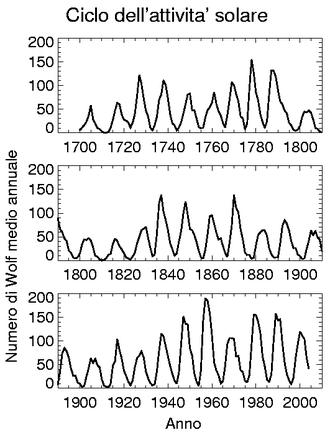
\includegraphics[width=\marginparwidth]{figures/chap1/1_4_macchie.png}}
	\caption{\scriptsize Andamento delle macchie solari (wikipedia).}
        \label{fig:1_4_macchie-png}
    }
    Un SD a tempi discreti può essere realizzato con l'osservazione delle macchie solari ogni 6 mesi. \\
    Nella pratica si ottengono degli andamenti come in Figura \ref{fig:1_4_macchie-png}.
\end{exmp}
\noindent
\begin{exmp}[Andamento degli individui di una popolazione, modello lineare.]
    \label{ex:pop_lin}
   Prendiamo una popolazione di individui descritta dallo stato $N_i$: il numero di individui al tempo $t=i \ \in \mathbb{N}$. \\
   La dinamica dello stato è descritta dal legame tra $N_i$ e $N_{i-1}$. Nota questa legge è possibile predire i futuri andamenti della popolazione.\\
   Il modello più semplice da studiare è il \textbf{modello lineare}:
   \[
       N_n = r N_{n-1} \qquad r \in \mathbb{R}^+
   .\] 
   Ipotizzando che il numero di individui all'istante iniziale (arbitrario) sia $N_0$ è possibile ricostruire una legge temporale che lega l'istante iniziale all'istante $n$:
   \[
       N_1 = rN_0; \qquad N_2 = rN_1=r^2N_0 \qquad \implies \qquad N_n = r^{n}N_0
   .\] 
   Quindi lo stato $n$-esimo è definito tramite una \textit{rete deterministica} legata allo stato iniziale.
   \marginpar{
       \captionsetup{type=figure}
           \incfig{1_5}
       \caption{\scriptsize Andamento della soluzione $N$ al variare del parametro $r$.}
       \label{fig:1_5}
   }
   Dalla Figura \ref{fig:1_5} si può osservare come l'andamento delle soluzioni dipende esclusivamente dal parametro $r$: sono possibili soltanto 3 casi.\\
   Il modello lineare è il più semplice che si possa costruire per studiare le popolazioni e, per quasi tutti i casi, non basta a spiegare i fenomeni fisici che ci circondano: è necessario elaborare un modello più complesso\ldots
\end{exmp}
\noindent
\paragraph{Principio di sovrapposizione}%
\label{par:Principio di sovrapposizione}
Riprendiamo l'Esempio \ref{ex:pop_lin}, abbiamo concluso che l'andamento dello stato del sistema (la popolazione) seguiva la legge:
\[
    N_n = r^nN_0
.\] 
Ipotizziamo che l'analisi prenda in considerazione l'andamento di due distinte popolazioni che seguono tale legge:
\[
    N_n = r^nN_0; \qquad M_n = r^nM_0
.\] 
Se lo studio prevede che queste due popolazioni si uniscano\sidenote{\scriptsize ad esempio per qualche ragione fisica, come la convivenza sullo stesso territorio} allora si ottiene la nuova popolazione $\overline{N}$:
\[
    \overline{N}_n = N_n + M_n = r^n(N_n + M_n) = r^n \overline{N}
.\] 
\begin{thm}[Principio di sovrapposizione.]
    Dati due sistemi che evolvono linearmente con la stessa legge: l'evoluzione della somma dei due ha lo stesso andamento della evoluzione dei singoli. 
\end{thm}
\noindent
Cosa avviene se i due sistemi non evolvono linearmente?
\subsection{Introduzione al Modello Logistico}%
\label{sub:Introduzione al Modello Logistico}
Prendiamo il seguente modello di popolazione:
\[
    N_{n+1} = r(N_n)\cdot N_n
.\] 
A differenza dell'esempio \ref{ex:pop_lin} il rate della popolazione $r$ adesso non è costante: dipende dalla popolazione all'istante $n$.\\
Un caso particolare di questa classe di sistemi è stato al centro di molti studi, in particolare per la sua versatilità nel modellizzare sistemi in ogni branca scientifica:
\begin{defn}[Modello logistico]
    Il modello logistico descrive l'andamento di una popolazione $N_n$ con il seguente rate $r$:
    \marginpar{
        \captionsetup{type=figure}
            \incfig{1_6}
        \caption{\scriptsize Andamento del Rate in funzione della popolazione, notiamo l'antimonotonia di $r$ che garantisce il fenomeno di retroazione.}
        \label{fig:1_6}
    }
    \[
	r(N_n) = \mu\left(1-\frac{N_n}{k}\right) 
    .\] 
    Quindi lo stato del sistema si esprime con la legge:
    \[
        N_{n+1} = \mu\left(1-\frac{N_n}{k}\right)N_n
    .\] 
    Questo rappresenta un modello non lineare.
\end{defn}
\noindent
Nel modello logistico la dipendenza di $r$ dalla popolazione permette un meccanismo di retroazione che sfavorisce la crescita della popolazione stessa.
\begin{exmp}[Modello logistico a popolazioni stellari.]
    Il modello logistico può essere utilizzato come "toy model" per descrivere il fenomeno di formazione delle stelle del tipo "Supernovae Triggered": 
    stelle che nascono in seguito all'esplosione di supernovae. \\
    Il modello prevede che le stelle neonate si trasformino in supernovae (al termine della loro vita) diventando anche loro sorgenti di stelle.
    \marginpar{
        \captionsetup{type=figure}
            \incfig{1_7}
        \caption{\scriptsize Porzione di spazio considerata per il modello, la stella con il contorno rosso è una stella in procinto di esplodere. $M$ è la quantità di materia totale all'interno di tale spazio, composta da stelle formate e gas interstellare.}
        \label{fig:1_7}
    }\\
    Ipotizziamo che ad un istante $i$ la popolazione di stelle sia $S_i$ e la massa del gas interstellare sia $M$. Tutte le stelle del modello hanno la stessa massa $m$ e sono identiche. \\
    Vogliamo modellare la popolazione stellare ad un istante successivo: $i+1$.\\
    La quantità di gas insterstellare disponibile (per la formazione di altre stelle) al tempo $t$ è data dalla massa totale $M$ meno la massa delle stelle presenti in tale istante:
    \[
        m_{\text{gas}} = M-S_i\cdot m
    .\] 
    Quindi il numero di stelle al tempo $i+1$ può essere espresso tramite un modello logistico:
    \[
	S_{i+1} = cS_i (M-S_i\cdot m)
    .\] 
    Cambiando variabili si arriva ad un sistema avente una notazione "classica" nello studio dei modelli logistici:
    \[
	x_i = \frac{mS_i}{M} \qquad r = \frac{cM}{4} \qquad \implies  \qquad x_{i+1} = 4rx_i(1-x_i)
    .\] 
\end{exmp}
\noindent
\subsection{Definizione Formale di Sistema Dinamico}%
\label{sub:Definizione Formale di Sistema Dinamico}
\paragraph{Spazio metrico}%
\label{par:Spazio metrico}
Prima di generalizzare le definizioni si SD è necessario definire uno spazio metrico:
\begin{defn}[Spazio metrico]
    L'inseme $X$ è spazio metrico se $\exists \ d:$ 
    \[
        d: \ X\times X \to \mathbb{R}^+ \cup \left\{0\right\}
    .\] 
    Che soddisfa le seguenti proprietà:
    \[\begin{aligned}
	& d(x, y) \ge 0; && \qquad d(x, y) = d(y, x); \\
	& d(x, y) = 0 \iff x = y; && \qquad d(x, y) \le d(x, z) + d(z, y)
    .\end{aligned}\]
\end{defn}
\noindent
\begin{exmp}[Spazio metrico]
    Prendiamo l'insieme di funzioni:
    \[
	C(I) = \left\{f(x)| x \in I \subset \mathbb{R}; f \text{ continua}\right\}
    .\] 
    Possiamo definire una distanza $d$ come:
    \[
	d(f(x), g(x)) = \sup\limits_{x \in I}\left|f(x)- g(x)\right|
    .\] 
\end{exmp}
\noindent
\paragraph{Definizione di SD a tempo discreto}%
\label{par:Definizione di SD a tempo discreto}
\begin{defn}[SD a tempo discreto]
    Un sistema dinamico a tempo discreto è rappresentato da una mappa $G: X\to X$ tale che
    \begin{itemize}
        \item $G^{n+m} = G^n \circ G^m \ \forall n, m \in \mathbb{N}_0 \cup \left\{0\right\}$.
	\item Se $G$ è invertibile $\implies$ $G^{-n} = G^{-1}\circ G^{-1} \circ \ldots \circ G^{-1}$, in cui la composizione viene applicata $n$ volte.
	    In questo caso $n, m \in \mathbb{Z}$.
    \end{itemize}
\end{defn}
\noindent
\begin{exmp}[Shift Map]
    Un esempio astratto di SD a tempo discreto è la Shift Map. L'insieme di partenza è così composto:
    \[
	S_k = \left\{1, 2, \ldots, k\right\}; \qquad \text{Insieme di $k$ simboli}
    .\] 
    Ci concentriamo su $S_2$\sidenote{di fatto è uno spazio binario (a due simboli: 0,1)}, definiamo uno spazio $s$ come:
    \[
        s = \left(s_1, s_2, \ldots, s_{\infty}\right) \quad s_i \in S_2
    .\] 
    E chiamiamo l'insieme delle possibili stringhe $\Sigma_2$ 
    \[
        \Sigma_2 = \left\{s | s = \left(s_1, s_2 , s_3, \ldots\right); s_i \in \Sigma_2\right\}
    .\] 
    Su questo spazio definiamo un operatore $\sigma: \Sigma\to \Sigma$ tale che
    \[
	\sigma (s) = \left(s_2, s_3, s_4\ldots\right) \in \Sigma_2
    .\] 
    L'operatore $\sigma$ definisce, insieme allo spazio $\Sigma$,  il sistema dinamico.\\
    Siano $s, t \in \Sigma_2$, possiamo definire una distanza $d: \Sigma_2\times \Sigma_2\to \mathbb{R}^+ \cup \left\{0\right\}$ come:
    \[
	d(s, t) = \sum_{j=0}^{\infty} \frac{\left|s_j-t_j\right|}{2^j}
    .\] 
    Notiamo che questa quantità è limitata, infatti:
    \[
	d(s, t) \le \sum_{j=0}^{\infty} \frac{1}{2^j} = 2 \quad \forall \ t, s
    .\] 
    \begin{thm}[Continuità di $\sigma$]
	Dati lo spazio metrico $\Sigma_2$, la trasformazione $\sigma$ e la distanza $d$ allora la trasformazione $\sigma$ è continua.
    \end{thm}
    \noindent
    Cerchiamo i \textbf{punti fissi} della mappa iterata $n$ volte: $s \in \Sigma_2$ tale che
    \[
	\sigma^n(s) = s
    .\] 
    Nel nostro sistema i punti sono stringe. Utilizziamo la notazione per indicare le stringhe fisse: $s^{n, j}$. Il primo indice corrisponde al numero di iterazioni per il quale la stringa $s$ è punto fisso, il secondo indice corre tra tutte le possibili stringhe che sono fisse per la $n$-esima iterazione.
    \[
	\sigma^n(s^{n,j}) = s^{n,j} 
    .\] 
    Nel caso di $n=1$ abbiamo (sempre per la shift map):
    \[\begin{aligned}
	&s^{1,1} = (0,0,0\ldots,0)\\
	&s^{1,2} = (1,1,1,\ldots,1)
    .\end{aligned}\]
    Infatti shiftando verso sinistra la mappa queste due stringhe risultano invarianti.\\
    Nel caso di $n=2$  le stringhe invarianti sono:
    \[\begin{aligned}
	&s^{2,1} = (0,1,0,1\ldots) \equiv (\overline{01})\\
	&s^{2,2} = (1,0,1,0\ldots) \equiv (\overline{10})
    .\end{aligned}\]
    Non è un caso che, per entrambi i casi, le stringhe fisse presentino una periodicità negli elementi ($n$-periodicità).
\end{exmp}
\noindent
\paragraph{Definizione di SD a tempo continuo}%
\label{par:Definizione di SD a tempo continuo}
\begin{defn}[Sistema dinamico a tempo continuo]
    Sia $X$ uno spazio metrico e $\varphi_t$ ($t \in \mathbb{R}$ ) una famiglia di mappe definite da:
    \[
	\varphi_t: X\to X
    .\] 
    e tale per cui
    \begin{itemize}
	\item $\varphi_0 = \mathbb{I}$.
	\item $\varphi_{t+s}=\varphi_t \circ \varphi_s$.
    \end{itemize}
    Inoltre si possono distinguere due tipi di SD a tempo continuo:
    \begin{enumerate}
        \item $t\in \mathbb{R}^+ \implies$ Semi Dynamical System.
        \item $t\in \mathbb{R} \implies$ Dynamical System.
    \end{enumerate}
    Nel caso $2.$ la mappa è detta invertibile, infatti si ha che:
    \[
        \varphi_{s+t} = \varphi_0 = \mathbb{I} \iff s = -t
    .\] 
\end{defn}
\noindent
\begin{exmp}[Traslazione]
    Sia $\vect{y}\in \mathbb{R}^n$ fissato; $t\in \mathbb{R}$. La mappa per il sistema agisce negli spazi:
    \[
	\varphi_t: \mathbb{R}^n \to \mathbb{R}^n \quad \forall \vect{x} \in \mathbb{R}^n: \vect{x}  \to \varphi_t(\vect{x})
    .\] 
    Operativamente la mappa è:
    \[
	\varphi_t(\vect{x}) = \vect{x} + t\vect{y}
    .\] 
    La mappa trasla il vettore $\vect{x}$ di un fattore $t\vect{y}$, possiamo chiederci se questa rispecchia le proprietà di sistema dinamico:
    \begin{itemize}
	\item $\varphi_0(\vect{x})= \vect{x}$.
	\item $t, s \in \mathbb{R}$; 
	    \[
		\varphi_s(\vect{x}) = \vect{x}  + t\vect{y}  \qquad \varphi_t(\vect{x}) = \vect{x}  + t\vect{y}
	    .\] 
	    \[\begin{aligned}
		\varphi_t(\vect{x}) \circ \varphi_s(\vect{x}) =& \ \varphi_t(\varphi_s)(\vect{x}) = \\
							       =& \ \vect{x} + s\vect{y} + t\vect{y} = \varphi_{t+s}(\vect{x})
	    .\end{aligned}\]
    \end{itemize}
\end{exmp}
\noindent
\paragraph{Soluzione, grafico e orbita di SD a tempi continui}%
\label{par:Soluzione, grafico e orbita di SD a tempi continui}
Si dice sistema dinamico autonomo un SD a tempi continui indipendente in modo esplicito dal tempo:
\[
    \frac{\text{d} \vect{x}}{\text{d} t} = F(\vect{x}, t) \qquad \vect{x}\in \mathbb{R}^n, F:\mathbb{R}^n\to \mathbb{R}^n
.\] 
Per gli insiemi di appartenenza si è usata la notazione semplificata.\\
Viceversa un sistema non autonomo:
\[
    \frac{\text{d} \vect{x}}{\text{d} t} =F(\vect{x}, t) \qquad 
    \vect{x}\in \mathbb{R}^n, t \in I \subset \mathbb{R}, F:\mathbb{R}^n\to \mathbb{R}^n
.\] 
Supponiamo di avere il seguente problema alle condizioni iniziali
\[\begin{aligned}
    & \frac{\text{d} \vect{x}}{\text{d} t} = F(\vect{x} ,t)\\
    & \vect{x} (t=0) = \vect{x}_0
.\end{aligned}\]
e supponiamo che la soluzione esista.
\begin{defn}[Soluzione del problema alle C.I.]
    La soluzione del problema alle condizioni iniziali $x (t, t_0, \vect{x}_0)$ è chiamata:
    \begin{itemize}
        \item Traiettoria per $\vect{x}_0$.
	\item Curva di Fase.
    \end{itemize}
    Ed ha l'ovvia proprietà:
    \[
	x(t, t_0, \vect{x}_0): \qquad x (t_0, t_0, \vect{x_0}) = \vect{x}_0
    .\] 
\end{defn}
\noindent
\begin{defn}[Grafico]
    Si definisce grafico della soluzione del problema alle CI l'insieme:
    \[
	\Gamma (\vect{x}_0) = \left\{(\vect{x}, t) \in \mathbb{R}^n \times \mathbb{R} | \ \vect{x}  = x(t, t_0, \vect{x}_0)\right\}
    .\] 
\end{defn}
\noindent
\begin{defn}[Orbita]
    Si definisce orbita della soluzione del problema alle CI:
    \[
	O(\vect{x}_0) = \left(\vect{x}\in \mathbb{R}^n | \ \vect{x}  = x(t, t_0, \vect{x}_0)\right)
    .\] 
\end{defn}
\noindent
\begin{exmp}[Oscillatore armonico]
    \marginpar{
        \captionsetup{type=figure}
            \incfig{1_8}
        \caption{\scriptsize Soluzione, grafico e orbita per l'oscillatore armonico.}
        \label{fig:1_8}
    }
    \[
        \begin{cases}
	    & \dot{u} = v\\
	    & \dot{v} = -u\\
	    & u_0 = 1\\
	    & v_0 = 0
        \end{cases}
    .\] 
    La variabile e le condizioni iniziali del problema sono:
    \[
	\vect{x}  = \begin{pmatrix} u(t)\\ v(t) \end{pmatrix} ; \quad \vect{x}_0 = \begin{pmatrix} 1 \\ 0 \end{pmatrix} 
    .\] 
    Si può dimostrare (\textcolor{mygreen}{esercizio}) che la soluzione è:
    \[
	x(t, t_0, \vect{x}_0) = \begin{pmatrix} \cos t \\ \sin t \end{pmatrix} 
    .\] 
\end{exmp}
\noindent
\subsection{Linearità di un Sistema Dinamico}%
\label{sub:Linearità di un Sistema Dinamico}
Prendiamo un sistema dinamico a tempi continui così definito:
\begin{equation}
    \frac{\text{d} \vect{x}}{\text{d} t} = F(\vect{x}, t) \qquad \vect{x}  \in \mathbb{R}^n; t \in \mathbb{R}; F: \mathbb{R}^n\times \mathbb{R} \to \mathbb{R}^n
    \label{eq:3_SD_cont}
\end{equation}
\[
    \vect{x}  = \left(x_1, x_2, \ldots, x_n\right) \qquad F = (F_1, F_2, \ldots, F_n)
.\] 
\begin{defn}[Condizione di linearità]
    \label{def:cond_lin}
    Un SD a tempi continui come quello di equazione \ref{eq:3_SD_cont} è lineare se:
    \[
	F(\vect{x}  + \vect{y}, t) = F(\vect{x}, t) + F(\vect{y}, t) \qquad \forall \vect{x}, \vect{y}  \in \mathbb{R}^n
    .\] 
\end{defn}
\noindent
Questa condizione è sufficiente ma non necessaria.
\begin{exmp}[Circuito RC]
    \marginpar{
        \captionsetup{type=figure}
        \fbox{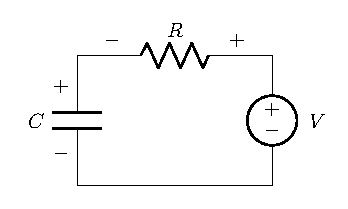
\includegraphics[width=\marginparwidth]{figures/tikz/3_rlc.pdf}}
        \caption{\scriptsize Circuito RC.}
        \label{fig:tikz-3_rlc-pdf}
    }
    Prendiamo il circuito RC come in figura \ref{fig:tikz-3_rlc-pdf}, l'equazione che regola la carica nel circuito è la seguente:
    \[
        \frac{\text{d} q}{\text{d} t} = \frac{V}{R}-\frac{q}{RC}
    .\] 
    In questo caso la variabile $x$ corrisponde con la carica.\\
    Il sistema non rispetta la condizione \ref{def:cond_lin}, infatti nello sviluppare il calcolo per due correnti, $q_1$ e $q_2$, rimane un termine $2V / R$. \\
    Nonostante questo il sistema è ancora lineare.
\end{exmp}
\noindent
\begin{exmp}[Pendolo]
    \marginpar{
        \captionsetup{type=figure}
            \incfig{1_9}
        \caption{\scriptsize }
        \label{fig:1_9}
    }
    Prendiamo il sistema del pendolo classico, le equazioni del moto della massa $m$ sono:
    \[
	\frac{\text{d} ^2\theta}{\text{d} t^2} = -\frac{g}{l}\sin\theta \implies
        \begin{cases}
	    \frac{\text{d} \theta}{\text{d} t} = y\\
	    \frac{\text{d} y}{\text{d} t} = - \frac{g}{l}\sin\theta
        \end{cases}
    .\] 
    Questo sistema è non lineare (c'è il seno).
\end{exmp}
\noindent
\begin{defn}[Criterio generale per la linearità]
    Un SD si dice lineare se la sua dipendenza dalle variabili di stato è lineare.
\end{defn}
\noindent

\input{lezioni/chap1/2_EsistenzaUnicitàSolIVP.tex}
\section{Introduzione ai Manifold}%
\label{sub:Introduzione ai Manifold}
Abbiamo fin'ora affermato che lo stato di un sistema dinamico è descritto da un vettore di $\mathbb{R}^n$, in questa sezione cerchiamo di essere più precisi riguardo a questa quantità.
\begin{exmp}[Pendolo nello spazio delle fasi]
    \[
        \begin{cases}
            \frac{\text{d} \theta}{\text{d} t} = y\\
	    \frac{\text{d} y}{\text{d} t} = -\frac{g}{l}\sin\theta
        \end{cases}
    \] 
    In questo caso abbiamo che lo stato $\vect{x} = (\theta, y)$ non è un vettore di $\mathbb{R}^n$ generico: $\theta$ è un angolo, $y$ è una velocità angolare.\\
    Lo stato è descritto in $\mathbb{R}^2$, la dinamica del sistema giace su una superficie dello spazio delle fasi detto \textbf{Manifold}.\\
    Il manifold per il problema del pendolo è una superficie cilindrica, si ha infatti che $\theta\in S_1$ e $y \in \mathbb{R}$ con $S_1$ cerchio di raggio unitario.
\end{exmp}
\noindent
\begin{defn}[Omomorfismo]
    Sia $h: U\to V$ con $U, V \subset \mathbb{R}^n$. Supponiamo che $\exists \ h^{-1}$, allora $h$ è omomorfismo se $h$ e $h^{-1}$ sono entrambe continue.
\end{defn}
\noindent 
\begin{defn}[Diffeomorfismo $C^r$]
    Siano $U, V \subset \mathbb{R}^n$ e $F:U\to V$. Diciamo che $F$ è un diffeomorfismo $C^r$ ($r\ge 1$) se esiste $F^{-1}$ e inoltre sia $F$ che $F^{-1}$ sono entrambe $C^r$ (derivata continua fino all'ordine $r$).
\end{defn}
\noindent
\begin{defn}[Manifold n-dimensionale]
    Sia $M \in \mathbb{R}^N$, diciamo che $M$ è un $K$ Dimensional Manifold se ($K<N$) se:
    \begin{itemize}
	\item $\forall m \in M $ esiste un \textbf{Intorno aperto} $W_i$ di esso con la proprietà: $M = \bigcup_i W_i$.
	\item $\forall W_i$ esiste un omomorfismo $\phi_i: W_i \to V_i \subset \mathbb{R}^N$.
	\item Se $W_i \cap W_j \neq 0$ la mappa $\phi_i \circ \phi_j = c_{ij}$  definita in $\phi_j(W_i \circ W_j)$ è un diffeomorfismo $C^r$ ($r\ge 1$).
    \end{itemize}
\end{defn}
\noindent
Ogni coppia $(W_i, \phi_i)$ è detta \textcolor{red}{Carta}, mentre l'insieme di tutte le carte $\left\{(W_i, \phi_i) \right\}$ è detto \textcolor{red}{Atlante}.\\
La cosa importante è che tramite i funzionali $\phi$ è possibile introdurre le proprietà di differenziabilità sul manifold utilizzando le definizioni di differenziabilità su $\mathbb{R}^N$ (euclidee) che sono ben definite.
\begin{figure}[H]
    \centering
    \fbox{\import{./figures/chap1/}{3_2.pdf_tex}}
    \caption{\scriptsize Azione dell'omomorfismo sul manifold.}
    \label{fig:3_2}
\end{figure}
\subsection{Mappare la dinamica di un Manifold in uno spazio euclideo $\mathbb{R}^K$}%
\label{sub:Mappare la dinamica di un Manifold in Rn }
Supponiamo di avere la mappa $G: W_i\to W_i$, ovvero manda punti del sottoinsieme $W_i$ (un intorno del punto $m$) del Manifold in punti di $W_i$.\\
Prendiamo $\vect{x}_1 \in W_i$: $\vect{x}_2 = G(\vect{x}_1)\in W_i$.\\
Possiamo mappare la $G$ in $\mathbb{R}^K$ nel seguente modo:
\[
    \vect{y}_1 = \phi_i(\vect{x}_1); \qquad \vect{y}_2 = \phi_i(\vect{x}_2)
.\] 
I punti $\vect{y}_{1,2}$ appartengono a $\mathbb{R}^K$. Il modo in cui si trasporta la differenziabilità all'interno del manifold è il seguente:
\[
    \vect{y}_2 = \phi_i(G(\vect{x}_1)) = \phi_i(G(\phi_i^{-1}(\vect{y}_1)))
.\] 
Visto che $\phi_i$ e $G$ sono note, che $\phi_i$ è omomorfismo e che $\vect{y}_1, \vect{y}_2 \in \mathbb{R}^K$ abbiamo che le proprietà di diff. sono applicabili ai funzionali sul manifold nello stesso modo in cui le applichiamo su $\mathbb{R}^K$. Inoltre si ha che:
\[
    \v{y}_2 = \phi_i \circ G \circ \phi_i^{-1}(\v{y}_1) 
.\] 
Definisce l'evoluzione dinamica del sistema su $\mathbb{R}^K$ .

\section{Mappe Ricorsive}%
\label{sub:Mappe Ricorsive}
Ricordiamo che una mappa ricorsiva è definita da:
\[
    \vect{x}_{n+1} = G(\vect{x}_n) \qquad \vect{x}_n \in \mathbb{R}^n; \qquad G:\mathbb{R}^n\to \mathbb{R}^n
.\] 
\begin{enumerate}
    \item La mappa è invertibile se $\exists \ G^{-1}$.
    \item La mappa è $C^r$ se esistono e sono continue le derivate\sidenote{\scriptsize Intese come parziali in più dimensioni} di $G$ fino all'ordine $r$.
\end{enumerate}
Se valgono la $1)$ e la $2)$ allora si ha un \textbf{Diffeomorfismo} $C^r$.
\subsection{Orbita per mappa ricorsiva invertibile}%
\label{sub:Orbita per mappa ricorsiva invertibile}
Se la mappa è invertibile allora preso un punto $\vect{x}_0$ è possibile muoversi verso destra (con $G$) o verso sinistra con $G^{-1}$.
\[
    \ldots, \ G^{-1}(\vect{x}_0), \ G^{-1}(\vect{x}_0), \ \vect{x}_0, \ G(\vect{x}_0), \ G^2(\vect{x}_0), \ \ldots
.\] 
\begin{exmp}[Mappa lineare]
    \[
        x_{n+1} = a x_n \qquad a \in \mathbb{R} - \left\{0\right\}
    .\] 
    Questa mappa è invertibile: basta spostare il parametro $a$ a sinistra per ricavare la preimmagine.
\end{exmp}
\noindent
Le mappe più studiate sono quelle non invertibili, questo perché al variare dei loro parametri si possono generare dei comportamenti particolari (caos).\\
Ci sono casi in cui anche le mappe all'apparenza invertibili possono generare situazioni complicate, ad esempio quelle che presentano un modulo come vedremo negli esempi di questa sezione.
\subsection{Orbita per mappa ricorsiva non invertibile}%
\label{sub:Orbita per mappa ricorsiva non invertibile}
Preso un punto $\vect{x}_0$ per una mappa non invertibile è possibile spostarsi soltanto verso destra tramite la $G$.
\[
    \vect{x}_0, \ G(\vect{x}_0), \ G^2(\vect{x}_0), \ \ldots
.\] 
\begin{exmp}[Mappa logistica]
    \[
        x_{n+1} = 3.5 x_n \left(1- x_n\right) \qquad x_n \in \left[0,1\right]
    .\] 
    Questa mappa non è invertibile: la preimmagine non è univoca (un'equazione del secondo grado ha due soluzioni).
\end{exmp}
\noindent
\begin{exmp}[Mappa di Bernoulli]
    \[
	x_{n+1}=2x_n \quad \text{mod}(1)
    .\] 
    Questa mappa è parente della shift-map poiché, scegliendo di rappresentare $x$ in base due, la mappa agisce allo stesso modo sui coefficienti della espansione (di base due) di come agiva con i simboli la shift map.
    \marginpar{
        \captionsetup{type=figure}
            \incfig{4_1}
        \caption{\scriptsize Mappa di Bernoulli, si vede come la linea rossa non rappresenti una funzione iniettiva: non può essere invertibile.}
        \label{fig:4_1}
    }\\
    L'operazione di modulo $1$ invece si occupa di traslare in $[0,1]$ il punto $x_{n+1}$ ogni volta che esce dall'intervallo a causa all'applicazione della mappa. \\
    L'operazione di traslazione avviene tramite un intero $n$ tale che:
    \[
	n = \text{min}(k \in \mathbb{Z}): \ 0 \le x+n \le 1
    .\] 
    Pur essendo lineare (all'apparenza) questa mappa può esibire un comportamento complesso. La presenza del modulo infatti fa si che la mappa non sia invertibile, come si può vedere in figura \ref{fig:4_1}.
\end{exmp}
\noindent
    \begin{exmp}[Circle Rotation Map]
	Prendiamo una classe di mappe generale del seguente tipo:
        \[
	    x_{n+1} = G(x_n) \qquad x_n \in S_1
        .\] 
	$S_1$ rappresenta il cerchio di raggio unitario, quindi i punti della mappa appartengono tutti al cerchio e sono rappresentati da una variabile: l'angolo di rotazione $x\cdot 2\pi$ (con $x \in \left[0,1\right]$).
	\marginpar{
	    \captionsetup{type=figure}
	        \incfig{4_2}
	    \caption{\scriptsize Rappresentazione della Circle Rotation Map.}
	    \label{fig:4_2}
	}\\
	La Circle Rotation Map è un caso particolare di queste mappe, ovvero:
	\[
	    x_{n+1}=x_n+\alpha  \quad \text{mod}(1); \qquad \alpha\in [0,1[
	.\] 
	La caratteristica principale di questa mappa è che può essere:
	\begin{itemize}
	    \item \textbf{$k$-periodica} se $\alpha$ razionale: le orbite degli $x_n$ si richiudono.
	    \item \textbf{Quasi periodica} se $\alpha$ irrazionale: i punti della mappa si distribuiscono uniformemente sul cerchio unitario (questo è il caso mostrato in figura \ref{fig:4_2}).
	\end{itemize}
	La mappa è sempre invertibile. 
\end{exmp}
\noindent
\begin{exmp}[Mappa di Arnold]
        \[
	    x_{n+1} = x_n + \omega  - \frac{k}{2\pi}\sin (2\pi x_n) \qquad \text{mod}(1) 
        .\] 
	$k, \omega$ sono costanti e $k>0$, la mappa non è lineare a causa della presenza del $\sin$.\\
	Il parametro $\omega$ può essere interpretato come il rapporto tra due frequenze: una intrinseca del sistema ed una forzante esterna.
	\[
	    \omega  \sim \frac{\omega_{\text{int}}}{\omega_{\text{ext}}}; \qquad \omega \in \left[0,1\right]
	.\]
	La mappa mostra le seguenti peculiarità:
	\begin{itemize}
	    \item $0\le k\le 1$: la mappa di comporta come la Circle Map, presenta orbite periodiche o quasi periodiche a seconda della razionalità di $\omega$. 
	    \item $k>1$: la mappa può esibire comportamenti caotici.
	\end{itemize}
	Nel caso di $k=1$ la mappa inizia a riscontrare alcune "anomalie", è il valore per il quale iniziano a rompersi le "lingue di Arnold".
\end{exmp}
\noindent
\begin{ex}[Sulla mappa di Arnold]
       Dimostrare che la mappa di Arnold è invertibile se $0\le k\le 1$.\\
       \textbf{Soluzione}:
       \marginpar{
           \captionsetup{type=figure}
           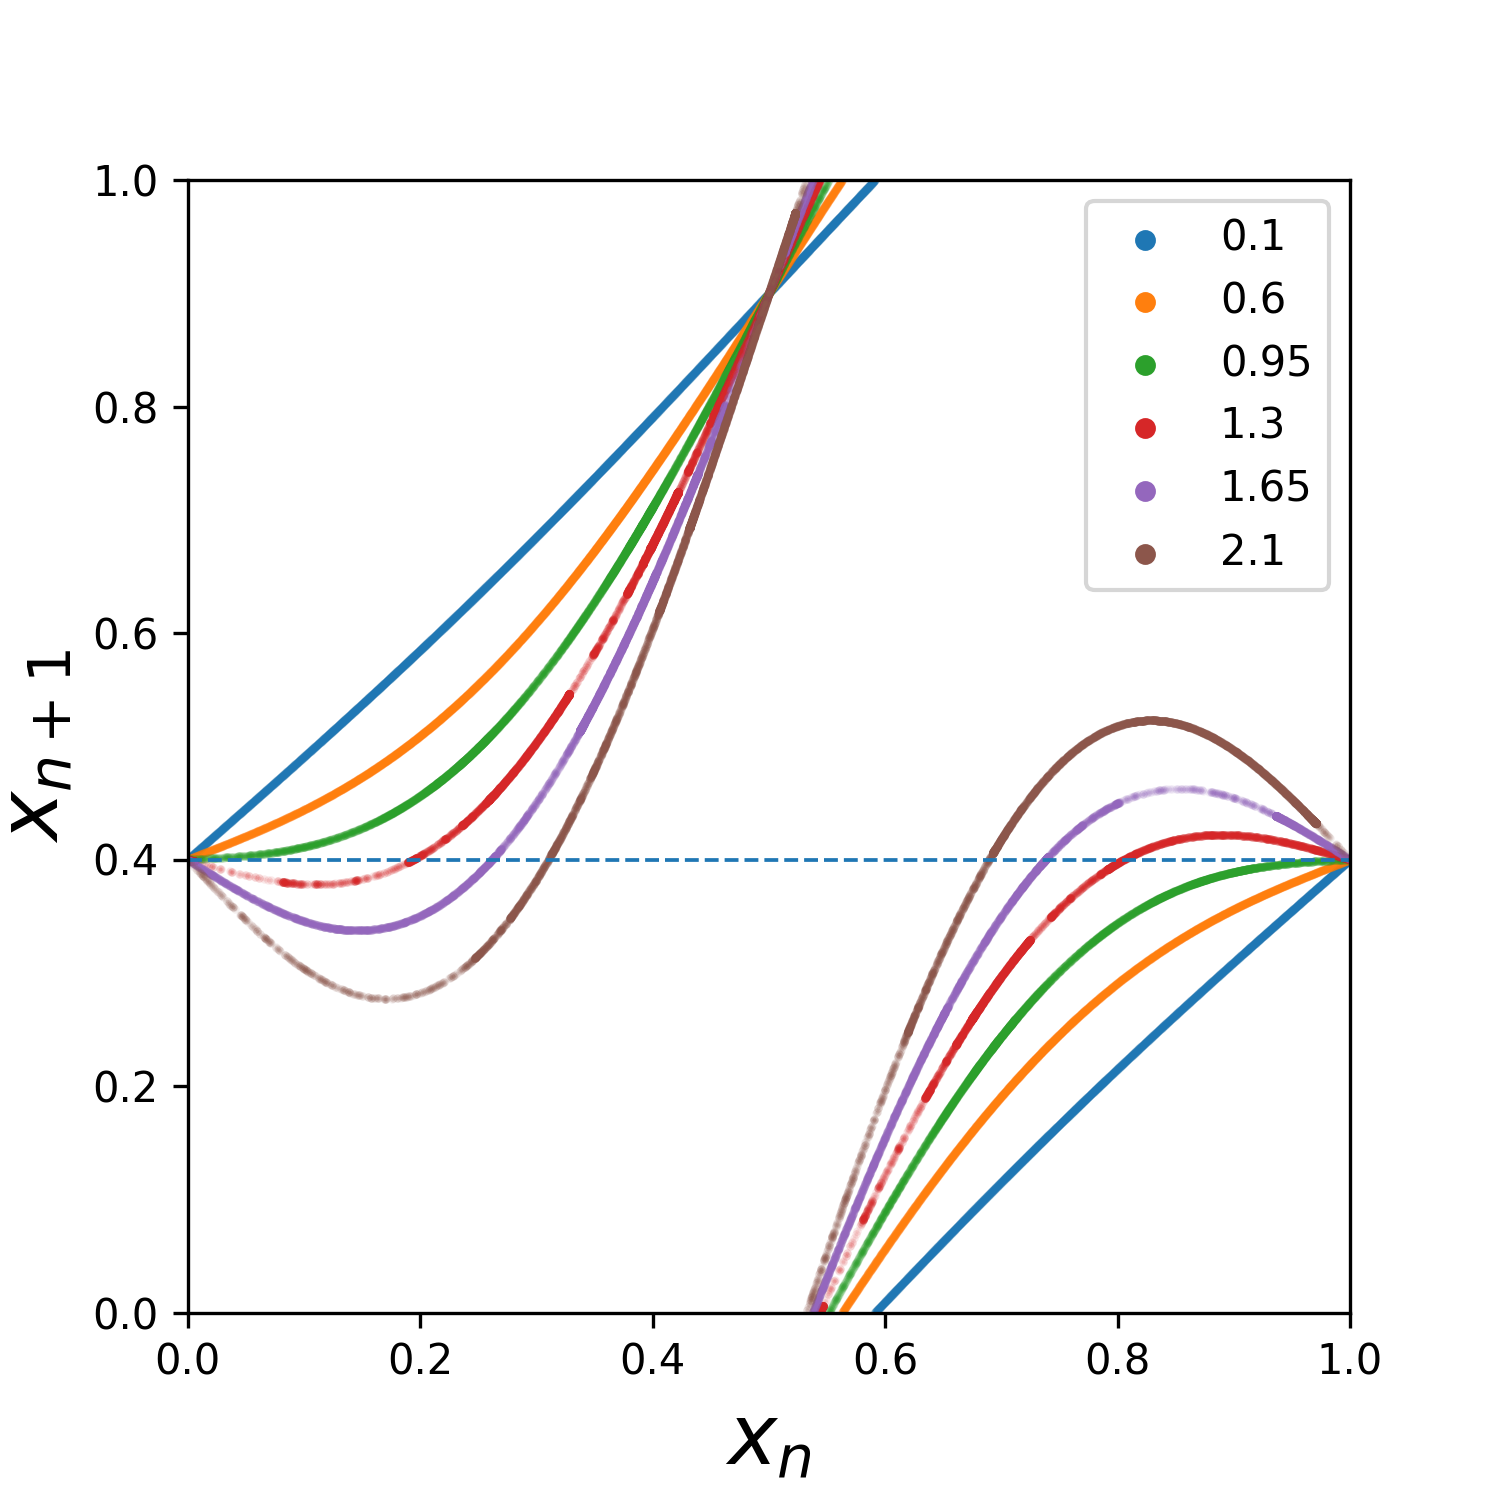
\includegraphics[width=\marginparwidth]{figures/4_3_py.png}
	   \caption{\scriptsize Mappa di Arnold al variare di $k$ con $\omega  = 0.4$ fissato.}
           \label{fig:4_3_py-png}
       }
       Come possiamo vedere in figura \ref{fig:4_3_py-png} la mappa non presenta criticità (è invertibile) se non nell'intorno di $x_n=0$ oppure $x_n=1$. \\
       Prendiamo ad esempio la mappa con $k=0.1$ e valutiamo\sidenote{\scriptsize Questa corrisponde (circa) alla circle rotation map} il punto $x_n=0$: la linea rossa, che rappresenta la mappa, a destra di questo punto vale $\omega+\epsilon$, a sinistra di questo punto vale $\omega-\epsilon$. La pendenza della curva in questo punto è quindi positiva.\\
       La presenza della perturbazione oscillante fa si che i due "rami" della mappa si avvicinino l'un l'altro, di conseguenza se la perturbazione è abbastanza forte è possibile che in un punto tra $0$ e $1$ il ramo in alto e quello in basso abbiano la stessa $x_{n+1}$: si perde l'iniettività e quindi l'invertibilità.\\
       Nel grafico la perdita di iniettività si ha quando la mappa oltrepassa la linea tratteggiata (che rappresenta la separatrice tra i rami).\\
       Per capire quando questo succede possiamo studiare la pendenza della mappa nei pressi di $x_n = 0$ (considerandola di fatto come una funzione continua).
       \[
	   x_{n+1} = x_n + \omega + k x_n = (1-k) x_n + \omega
       .\] 
       Se in un intorno (destro) di questo punto la pendenza della curva è negativa allora significa che la mappa è scesa sotto $\omega$ e quindi ha perso l'iniettività: deve essere $k\le 1$ per avere pendenza positiva.
\end{ex}
\noindent


\section{Spazio delle fasi esteso (SD a tempi continui)}%
\label{sub:Spazio delle fasi esteso (SD a tempi continui)}
Si prende un sistema dinamico a tempi continui autonomo e lo si perturba con una componente dipendente dal tempo (un fattore esterno). Il sistema in questo modo diventa non autonomo, l'equazione generale che regola questo tipo di sistema è:
\[
    \frac{\text{d} \vect{x}}{\text{d} t} = F(\vect{x},t) \qquad \vect{x}\in \mathbb{R}^n; \ F: \mathbb{R}^n \times \mathbb{R}\to \mathbb{R}^n
.\] 
Possiamo ricondurre questo sistema ad un sistema autonomo tramite una trasformazione nella variabile temporale:
\[
    t = m(s) = s \implies  \frac{\text{d} }{\text{d} t} = \frac{\text{d} s}{\text{d} t} \frac{\text{d} }{\text{d} s} 
.\] 
Inserendo nella equazione del moto:
\[
    \frac{\text{d} \vect{x}}{\text{d} t} = \frac{\text{d} s}{\text{d} t} \frac{\text{d} \vect{x}}{\text{d} s} = F(\vect{x}, t)
.\] 
Possiamo definire il differenziale di $t$  rispetto a $s$: $dt /ds = 1$.
\[
    \begin{cases}
	\frac{\text{d} \vect{x} (s)}{\text{d} s} = F(\vect{x}, t)\\
	\frac{\text{d} t}{\text{d} s} = 1
    \end{cases}
\] 
\begin{defn}[Spazio delle fasi esteso]
    Si definisce spazio delle fasi esteso la quantità:
    \[
	\vect{y} =(\vect{x}, t) \in \mathbb{R}^n \times \mathbb{R}
    .\] 
\end{defn}
\noindent
In questo modo, definendo anche il funzionale esteso:
\[
    H = (F(\vect{x}, t), 1)
.\] 
Si possono generalizzare le equazioni del moto come:
\[
    \frac{\text{d} \vect{y}}{\text{d} s} = H(\vect{y})
.\] 
Per quanto il problema sia formalmente risolto si deve tenere in considerazione che il nuovo spazio delle fasi potrebbe non essere più un compatto.\\
Questa mancanza potrebbe diventare un problema nei nostri scopi in quanto siamo spesso interessati alla soluzione asintotica del sistema (che potrebbe smettere di esistere).\\
In ogni caso aggiungiamo che, se la forzante è periodica, il sistema può essere sempre gestito con questo metodo.
\begin{exmp}[Forzante oscillante]
    \[
	\frac{\text{d} ^2x}{\text{d} t^2} = -x + A\sin (\omega t)
    .\] 
    Come sempre si riporta l'equazione ad una di primo ordine:
    \[
        \begin{cases}
            \frac{\text{d} x}{\text{d} t} = y \\
	    \frac{\text{d} y}{\text{d} t} = -x + A \sin (\omega t)
        \end{cases}
    \] 
    Adesso si introduce la variabile $\theta (t)=\omega t$. Il nuovo sistema, con questa variabile, è descritto nello spazio delle fasi generalizzato e le equazioni sono le seguenti:
    \[
        \begin{cases}
            \frac{\text{d} x}{\text{d} t} = y\\
	    \frac{\text{d} x}{\text{d} t} = -x + A\sin\theta\\
	    \frac{\text{d} \theta}{\text{d} t} =\omega
        \end{cases}
    \] 
    Si noti che la variabile $\theta$ non è limitata, quindi lo spazio delle fasi non è più un compatto.
\end{exmp}
\noindent

\section{Flusso di fase}%
\label{sub:Flusso di fase}
Dato un sistema dinamico a tempo continuo in $\mathbb{R}^2$:
\[
    \frac{\text{d} \vect{x}}{\text{d} t} = A\vect{x}
.\] 
\[
    \vect{x} = \begin{pmatrix} x_1 \\ x_2 \end{pmatrix}  \qquad A = \begin{pmatrix} - \Gamma  & 0 \\ 0 & \Gamma \end{pmatrix}; \ \Gamma  \in \mathbb{R}
.\] 
Studiamone l'evoluzione risolvendo il problema alle condizioni iniziali:
\[
    \begin{cases}
        \frac{\text{d} x_1}{\text{d} t} = -\Gamma  x_1\\
	\frac{\text{d} x_2}{\text{d} t} = \Gamma x_2\\
	\vect{x} (0)=\vect{x}_0
    \end{cases}
\] 
La soluzione può essere espressa tramite il seguente vettore:
\[
    \vect{x} (t)= 
    \begin{pmatrix}  
	x_{10}e^{-\Gamma t}\\
	x_{20}e^{\Gamma t}
    \end{pmatrix} 
.\] 
Oppure possiamo scriverla in termini di matrice:
\[
    \vect{x} (t)=
    \begin{pmatrix} 
    e^{-\Gamma t} & 0 \\
    0 & e^{\Gamma t}
    \end{pmatrix} 
    \begin{pmatrix} 
	x_{10}\\
	x_{20}
    \end{pmatrix} 
    \equiv \varphi_t (\vect{x}_0)
.\] 
\begin{defn}[Flusso di fase]
    L'operatore $\varphi_t$ definito come
    \[
        \varphi_t: \mathbb{R}^2 \to \mathbb{R}^2; \quad 
	\varphi_t = 
	\begin{pmatrix} 
	    e^{-\Gamma t} & 0 \\
	    0 & e^{\Gamma t} 
        \end{pmatrix} 
    .\] 
    Si dice flusso di fase del sistema.
\end{defn}
\noindent
\paragraph{Proprietà del flusso di fase}%
\label{par:Proprietà del flusso di fase}
\begin{enumerate}
    \item $\varphi_t(\vect{x}_0)$ è una soluzione dell'IVP.
    \item $\varphi_0(\vect{x}_0) = \vect{x}_0$ 
    \item $\varphi_{t+s}(\vect{x}_0)=\varphi_t(\varphi_s(\vect{x}_0))$ 
\end{enumerate}
Notiamo che se $\varphi_t$  è invertibile allora il suo inverso è $\varphi_{-t}$.  
\begin{exmp}[Flusso unodimensionale]
    \[
        \begin{cases}
            \frac{\text{d} x}{\text{d} t} = x^2-1\\
	    x(0) = x_0
        \end{cases}
    .\] 
    Prima di ricavare il flusso di fase determiniamo la soluzione:
    \[
        \frac{dx}{x^2-1} = dt \implies  \frac{dx}{2} \left[\frac{1}{x-1}-\frac{1}{x+1}\right] = dt
    .\] 
    Integrando a destra e sinistra:
    \[
	\log (\frac{\left|x-1\right|}{\left|x+1\right|}) = 2t + c
    .\] 
    Per ricavare $x(t)$  è necessario uno studio di funzione all'interno del logaritmo per capire quando è necessaria una inversione di segno nel suo argomento.\\
    Per $\left|x\right| > 1$  l'argomento è positivo, possiamo procedere in tal caso a risolvere con l'elevamento a potenza:
    \[
        \frac{x-1}{x+1}=e^{2t}B
    .\] 
    La costante $B$  si determina imponendo la condizione iniziale $x(0)=x_0$:
    \[
        B=\frac{x_0-1}{x_0+1}
    .\] 
    In conclusione la soluzione è:
    \[
	x(t) = \frac{(x_0+1)+e^{2t}(x_0-1)}{(x_0+1) -e^{2t}(x_0-1)} = \varphi_t(x_0)
    .\] 
    In questo caso abbiamo un flusso che non è rappresentato da una matrice ma da un funzionale. Possiamo dimostrare che è un flusso: le prime due richieste sono ovvie. La terza invece è lasciata per esercizio, si tratta di fare tanti conti.
\end{exmp}
\subsection{Generalizzazione $n$ dimensionale}%
\label{sub:Generalizzazione $n$ dimensonale}
Prendiamo nuovamente la definizione di Flusso partendo dal solito sistema:
\[
    \begin{dcases}
	\frac{\text{d} \vect{x}}{\text{d} t} = F(\vect{x})\\
	\vect{x} (0)=\vect{x_0}
    \end{dcases}
    \qquad 
    F \in C^r, \ F:\mathbb{R}^n\to \mathbb{R}^n; \ \vect{x}_0 \in \mathbb{R}^n
.\] 
Possiamo caratterizzare la soluzione tramite il funzionale flusso:
\[
    \varphi (t,\vect{x}): \mathbb{R}^n\to \mathbb{R}^n
.\] 
L'applicazione del funzionale manda la variabile $\vect{x}$ nella soluzione, in questo modo il funzionale caratterizza completamente il sistema.\\
Le proprietà della $\varphi$ sono:
\begin{enumerate}
    \item $\varphi (t, \vect{x}) \in C^r$.
    \item $\varphi (0, \vect{x}_0) = \vect{x}_0$.
    \item $\varphi (t + s, \vect{x}_0) = \varphi (t, \varphi (s, \vect{x}_0))$.
\end{enumerate}
\subsection{Flusso di Fase per sistemi non autonomi}%
\label{sub:Flusso di Fase per sistemi non autonomi}
Introduciamo adesso il flusso nel caso in cui il sistema non è autonomo. Un sistema non autonomo è generalmente caratterizzato dalle equazioni:
\[
    \begin{dcases}
	\frac{\text{d} \vect{x}}{\text{d} t} = F(\vect{x}, t)\\
	\vect{x}(t_0) = \vect{x}_0
    \end{dcases}
    \qquad 
    \vect{x} \in \mathbb{R}^n; \ F \in C^r; \ F: \mathbb{R}^n\to \mathbb{R}^n
\] 
Notiamo che nella condizione iniziale si è messo come tempo iniziale $t_0$, questo è dovuto al fatto che, in un sistema non autonomo, la soluzione dipende dalla variabile $t_0$ (e non solo da $t-t_0$ come si avrebbe per un sistema autonomo). Questa caratteristica corrisponde alla perdita di invarianza per traslazione temporale della soluzione.\\
Le metodologie che permettono di introdurre il flusso in questi sistemi sono $2$:
\begin{itemize}
    \item Process Formulation.
    \item Skew Product Flow Formulation.
\end{itemize}
\paragraph{Process Formulation.}%
\label{par:Process Formulation.}
Supponiamo che esista e sia unica la soluzione del IVP e che tale soluzione sia globale (definita $\forall \ t$).\\
Definiamo il flusso di questo sistema come la soluzione dell'IVP $\Phi(t, t_0, \vect{x}_0)$. Le proprietà di $\Phi$  sono:
\begin{enumerate}
    \item $\Phi(t, t_0, \vect{x}_0)$ eredità tutte le proprietà del funzionale $F$.
    \item $\Phi(t_0, t_0, \vect{x}_0) = \vect{x}_0$ (Proprietà di identità).
    \item $\Phi(t_2, t_0, \vect{x}_0) = \Phi(t_2, t_1, \Phi(t_1, t_0, \vect{x}_0))$ con $t_0 \le t_1\le t_2$.
\end{enumerate}
Potremmo essere più formali definendo lo spazio:
\[
    \mathbb{R}^2_{\ge } \equiv \left\{ (t, t_0) \in \mathbb{R}^2 \ | \ t \ge t_0\right\}
.\] 
Quindi definiamo il flusso di fase come il funzionale (di variabile generica $*$):
\[
    \varphi (t,t_0,*):\mathbb{R}^n\to \mathbb{R}^n \qquad \text{con } (t, t_0) \in \mathbb{R}^2_{\ge }
.\] 
Che gode delle solide proprietà di flusso, che ripetiamo:
\begin{enumerate}
    \item $\varphi(t, t_0, \vect{x}_0) \in C^r$ con $r\ge 1$.
    \item $\varphi(t_0, t_0, \vect{x}_0) = \vect{x}_0$ (Proprietà di identità).
    \item $\varphi(t_2, t_0, \vect{x}_0) = \varphi(t_2, t_1, \varphi(t_1, t_0, \vect{x}_0))$ con $(t_2, t_1) \in \mathbb{R}^2_{\ge }$, e anche $(t_1, t_0) \in \mathbb{R}^2_{\ge }$ .
\end{enumerate}
\begin{exmp}[Flusso per Process Formulation]
    Prendiamo il sistema:
    \[
        \begin{dcases}
	    \frac{\text{d} x}{\text{d} t} = -2tx\\
	    x(t_0) = x_0
        \end{dcases}
    .\] 
    Si può dimostrare (esercizio) che la soluzione ha la forma:
    \[
	x(t)=x_0e^{-(t^2-t_0^2)} \equiv \varphi (t, t_0, x_0)
    .\] 
    La dipendenza da $t_0$ non può essere eliminata in questo caso con una traslazione temporale, questo è dovuto al fatto che l'argomento dell'esponenziale non è riscrivibile come funzione di $t-t_0$:
    \[
	t^2-t_0^2 = \left(t-t_0\right)^2 + 2(t-t_0)t_0
    .\] 
\end{exmp}
\noindent
\paragraph{Skew Product Flow Formulation}%
\label{par:Skew Product Flow Formulation}
L'idea alla base del metodo è quella di aggiungere ulteriori equazioni del moto in modo tale da rendere il sistema nuovamente autonomo. A quel punto il flusso di fase sarà quello già visto in precedenza.
\begin{exmp}[Pendolo]
    Nel caso del pendolo l'equazione del moto abbiamo visto che è:
    \[
	\ddot{x} = - x + A \sin (\omega t)
    .\] 
    E per rendere autonomo il sistema nuovamente abbiamo introdotto la variabile $\theta  = \omega t$. La chiave del funzionamento del metodo è proprio il fatto che $\theta$ ha una evoluzione autonoma.
\end{exmp}
\noindent
Formalmente prendiamo di nuovo il sistema di partenza:
\[
    \begin{dcases}
	\frac{\text{d} \vect{x}}{\text{d} t} = F(\vect{x}, t)\\
	\vect{x}(t_0) = \vect{x}_0
    \end{dcases}
    \qquad 
    \vect{x} \in \mathbb{R}^n; \ F \in C^r; \ F: \mathbb{R}^n\to \mathbb{R}^n
\]
Introduciamo un sistema dinamico da affiancare a questo:
\[
    \begin{dcases}
	\frac{\text{d} \vect{q}}{\text{d} t} = G(\vect{q})\\
	\vect{q} (t_0)= \vect{q}_0
    \end{dcases}
.\] 
Questo nuovo sistema è autonomo, possiamo allora risolvere il problema nel sistema di variabili:
\[
    \vect{y} =(\vect{x}, \vect{q}) \in \mathbb{R}^n \times \mathbb{R}^d
.\] 
Con $\mathbb{R}^d$ spazio di definizione di $\vect{q}$.
\[
    \begin{dcases}
	\frac{\text{d} \vect{x}}{\text{d} t} = F(\vect{x}, \vect{q})\\
	\vect{x} (t_0)=\vect{x_0}\\
	\frac{\text{d} \vect{q}}{\text{d} t} = G(\vect{q})\\
	\vect{q} (t_0)=\vect{q}_0
    \end{dcases}
.\] 
Il sistema in $\vect{q}$ è definito "Driver", il sistema in $\vect{x}$ invece è spesso detto "schiavizzato" dal Driver. Il sistema complessivo risulta comunque autonomo.\\
Quindi possiamo definire il flusso come lo spazio delle soluzioni in $\vect{x}$ e $\vect{q}$:
\[
    \varphi_t(\vect{x}_0, \vect{q}_0) = (\vect{x} (t, \vect{x}_0, \vect{q}_0), \vect{q} (t, \vect{q}_0))
.\] 
Essendo un sistema autonomo valgono le proprietà di flusso già viste:
\begin{enumerate}
    \item $\varphi_t \in C^r$ con $r\ge 1$.
    \item $\varphi_{t_0}(\vect{x}_0, \vect{q}_0) = (\vect{x}_0,\vect{q}_0)$.
    \item $\varphi_{t+s}(\vect{x}_0, \vect{q}_0) = \varphi_t(\varphi_s(\vect{x}_0, \vect{q}_0))$.
\end{enumerate}
Concentriamoci sulla terza proprietà ed esplicitiamola in modo diverso:
\[\begin{aligned}
    \varphi_{t+q} (\vect{x}_0, \vect{q}_0) =&  (\vect{x} (t+s , \vect{x}_0, \vect{q}_0), \vect{q} (t+s, \vect{q}_0)) = \\
                                           =& (\vect{x} (t, \vect{x} (s, \vect{x}_0,\vect{q}_0) \vect{q}(s, \vect{q}_0) ), \vect{q} (t, \vect{q} (s, \vect{q}_0)) ) = \\
					   =&(\vect{x} (t, \vect{x} (s, \vect{x}_0,\vect{q}_0),  \vect{q}(s, \vect{q}_0) ), \vect{q} (t+s, \vect{q}_0))
.\end{aligned}\]
Ed uguagliando la prima dopo l'uguale con l'ultima deve esser vero che:
\begin{defn}[Cocycle Property]
    \[
	\vect{x} (t+s, \vect{x}_0, \vect{q}_0) = \vect{x} (t, \vect{x} (s, \vect{x}_0, \vect{q}_0), \vect{q} (s, \vect{q}_0))
    .\] 
\end{defn}
\noindent
\begin{exmp}[Esempio di Cocycle Property]
    Prendiamo la seguente variabile "Driver":
    \[
	q(t) = t \in \mathbb{R} \qquad q(t_0)=t_0
    .\] 
    La proprietà in questo caso si esprime come:
    \[
	\vect{x} (t+s, \vect{x}_0, t_0) = \vect{x} ( t, \vect{x} (s, \vect{x}_0, t_0), t_0 + s)
    .\] 
\end{exmp}
\noindent

\section{Soluzioni speciali di Sistemi Dinamici}%
\label{sub:Soluzioni speciali di Sistemi Dinamici}
Analizziamo il regime asintotico di un sistema dinamico, i tipi di soluzione che si possono incontrare sono:
\begin{enumerate}
    \item Stati Stazionari Costanti.
    \item Stati Stazionari Dinamici.
	\begin{itemize}
	    \item Periodici.
	    \item Quasi Periodici.
	    \item Complessi.
	\end{itemize}
\end{enumerate}
\subsection{Stati Stazionari Costanti}%
\label{sub:Stati stazionari Costanti}
Questi stati sono indipendenti dal tempo, ipotizzando che la soluzione stazionaria si $\vect{x}(t)$ allora:
\[
    \vect{x} (t + \Delta t)=\vect{x} (t)
.\] 
Nei libri sono spesso chiamati Punti Singolari, Punti Critici, Soluzioni Stazionarie.
\subsection{Stati Stazionari Dinamici}%
\label{sub:Stati Stazionari Dinamici}
Lo stato per questi sistemi non è costante nel tempo, analizziamo le più comuni situazioni che si possono presentare in questi sistemi.
\paragraph{Orbite periodiche}%
\label{par:Orbite periodiche}
L'orbita di uno stato stazionario dinamico periodico è un'orbita che si ripete nel tempo.
\begin{exmp}[Oscillatore non lineare]
    \marginpar{
        \captionsetup{type=figure}
            \incfig{7_1}
        \caption{\scriptsize Orbita Periodica che attrae la dinamica nello spazio delle fasi.}
        \label{fig:7_1}
    }
    Un oscillatore non lineare è un sistema che presenta un'orbita periodica come in figura \ldots\\
    Se lo stato $\vect{x}_1$ si trova (con le condizioni iniziali) sull'orbita allora rimarrà su tale orbita a stazionarietà. Se uno stato $\vect{x}_2$ si trova invece in un altro punto dello spazio delle fasi inizialmente allora evolverà per raggiungere l'orbita stabile (a stazionarietà).
\end{exmp}
\noindent
\paragraph{Orbite quasi periodice}%
\label{par:Orbite quasi periodice}
Sono orbite che non si ripetono nel tempo, sono più complesse delle orbite periodiche. La loro struttura verrà approfondita nel seguito.
\paragraph{Comportamenti complessi}%
\label{par:Comportamenti complessi}
Quando un sistema presenta, ad esempio, caos deterministico.
\subsection{Orbite periodiche di sistema dinamico}%
\label{sub:Orbite periodiche di sistema dinamico}
\begin{defn}[Orbita periodica per SD a tempo continuo]
Prendiamo un Sistema Dinamico a tempo continuo:
\[
    \begin{dcases}
	\frac{\text{d} \vect{x}}{\text{d} t} = F(\vect{x}, t)\\
	\vect{x} (t_0) = \vect{x}_0
    \end{dcases}
    \qquad
    F: \ I \times \mathbb{R}^n \to \mathbb{R}^n
.\] 
 Sia $\vect{x}_p(t)$ la soluzione dell'IVP, diciamo che $\vect{x}_p(t)$ è periodica se:
\[
    \exists \ T \in \mathbb{R}^+: \ \vect{x}_p(t) = \vect{x}_p (t + T) \  \forall t \in I
.\]    
\end{defn}
\noindent
\begin{defn}[Orbita periodica per SD a tempo continuo]
    Dato un Sistema Dinamico a tempo discreto:
    \[
	\vect{x}_{k+1} = G(\vect{x}_k) \qquad \vect{x}_k \in \mathbb{R}^n
    .\] 
    Diciamo che $\vect{x}_p$ è una orbita $q$-periodica con $q \in \mathbb{N}$ se:
    \[
	G^{q} (\vect{x}_p) = \vect{x}_p
    .\] 
\end{defn}
\noindent
Prima di procedere definiamo la seguente categoria di funzioni:
\begin{defn}[Funzioni quasi periodiche]
    Una funzione $H$ si dice Quasi Periodica se può essere rappresentata nella seguente forma:
    \[
	H(t) = H(\omega_1t, \omega_2t, \ldots, \omega_nt)
    .\] 
    Con l'insieme di frequenze $\left\{\omega_i\right\}$ tra di loro Incommensurabili.\\
    Questo significa che non esiste una combinazione lineare di queste frequenze con coefficienti in $\mathbb{Q}$ che si annulla.
\end{defn}
\noindent
Preso un sistema a tempo continuo non autonomo e supponiamo di avere uno spazio delle fasi con un'orbita chiusa: l'orbita è necessariamente periodica? No.

\section{Campi Vettoriali e Proprietà dei SD a t. con. autonomi}%
\label{sub:Campi Vettoriali in SD a tempo continuo}
Prendiamo il solito sistema:
\[
    \begin{dcases}
	\frac{\text{d} \vect{x}}{\text{d} t} = F(\vect{x}, t)\\
	\vect{x} (t_0) = \vect{x}_0
    \end{dcases}
\] 
I campi di esistenza di tutte le quantità sono:
\[
    \vect{x}  \in \mathbb{R}^n; \quad F: I \times \mathbb{R}^n\to \mathbb{R}^n; \quad F \in C^r \ (r\ge 1)
.\] 
Assumiamo che le soluzioni siano definite globalmente, tale sistema dinamico viene spesso chiamato \textcolor{red}{Campo Vettoriale}.\\
Facciamo un esempio per capire da dove nasce l'idea che il sistema possa presentare un campo vettoriale.
\begin{exmp}[Campo Vettoriale in $\mathbb{R}^2$]
    \marginpar{
        \captionsetup{type=figure}
            \incfig{8_1}
	    \caption{\scriptsize Andamento della soluzione (ipotetica) e campo vettoriale nel punto $P$ che appartiene alla traiettoria.}
        \label{fig:8_1}
    }
    \[
        \begin{dcases}
	    \frac{\text{d} x_1}{\text{d} t} =F_1(x_1,x_2,t)\\
	    \frac{\text{d} x_2}{\text{d} t} = F_2(x_1, x_2, t)
        \end{dcases}
    \] 
    Supponiamo di aver trovato una soluzione particolare $\vect{x}_s(t)$ con condizioni iniziali $V_0 = (x_{10}, x_{20})$.\\
    Preso un punto appartenente alla soluzione (o orbita) $P(t, x_1, x_2)$ si ha che la tangente alla curva ha come componenti $\left.(F_1, F_2)\right|_{P}$. Questo vettore tangente definisce il campo vettoriale e può essere associato ad ogni punto dell'orbita.
\end{exmp}
\noindent
Dobbiamo aggiungere che, lo stesso sistema proiettato nello spazio delle fasi senza la componente temporale sarebbe una varietà schiacciata in due dimensioni. In questa proiezione può sembrare che le orbite si sovrappongano, questo in realtà non avviene: è dovuto all'aver effettuato una proiezione del moto reale.\\
Generalmente nel corso avremmo a che fare con SD autonomi.
\subsection{Proprietà dei sistemi dinamici a tempo continuo autonomi}%
\label{sub:Proprietà dei sistemi dinamici a tempo continuo autonomi}
Prendiamo il problema:
\[
	\frac{\text{d} \vect{x}}{\text{d} t} = F(\vect{x})
.\] 
Con le opportune condizioni iniziali e
\[
    F \in C^r \ (r\ge 1); \ x \in \mathbb{R}^n; \ F:\mathbb{R}^n\to \mathbb{R}^n
.\] 
Chiamiamo l'intervallo di esistenza della soluzione con il nome $I$.
\begin{thm}[Invarianza per Shift]
    Sia $\vect{x}_s(t)$ una soluzione dell'IVP per un SD a tempo continuo autonomo con le opportune condizioni iniziali. Allora: 
    \[
	\vect{x}_s(t+\tau) \text{ con } t + \tau  \in I 
    \] 
    è soluzione.
\end{thm}
\noindent
\begin{proof}
    Calcoliamo la quantità:
    \[
	\frac{\text{d} \vect{x}_s(t+\tau)}{\text{d} t} 
    .\] 
    Per vedere se corrisponde anch'essa alla soluzione del problema. La dimostrazione si conclude con il semplice cambio di variabili:
    \[
        t' = t + \tau  \implies  \frac{\text{d} }{\text{d} t} = \frac{\text{d} }{\text{d} t'} 
    .\] 
    Infatti inserendo nella equazione differenziale otteniamo:
    \[
	\frac{\text{d} \vect{x}_s(t')}{\text{d} t'} = F(\vect{x}_s(t'))
    .\] 
    Che ci dice appunto che la soluzione traslata è ancora soluzione.
\end{proof}
\begin{ex}[Su campo vettoriale]
    Preso il seguente campo vettoriale:
    \[
	\frac{\text{d} x}{\text{d} t} = - (1+x^2)
    .\] 
    e sia $x(t_0)=x_0$.
    \begin{itemize}
        \item Verificare che una soluzione è:
	    \[
		x(t)=- \tan(t-t_0-\arctan (x_0))
	    .\] 
	\item Verificare che $x(t+\tau)$ è ancora soluzione.
    \end{itemize}
\end{ex}
\noindent
\begin{ex}[Teorema di Shift e sistemi non autonomi 1]
    Preso il sistema
    \[
	\frac{\text{d} x}{\text{d} t} = e^t; \qquad  x(0)=x_0
    .\] 
    Dimostrare che la soluzione è:
    \[
	x(t)=e^t-1+x_0
    .\] 
    e verificare che il teorema di invarianza per shift non è verificato.
\end{ex}
\noindent
\begin{ex}[Teorema di Shift e sistemi non autonomi 2]
   Dato il sistema 
   \[
       \frac{\text{d} \vect{x}}{\text{d} t} = F(\vect{x}, t); \qquad \text{Soluzione: }\vect{x}_s(t)
   .\] 
   Verificare che, posti $\vect{x}_{\tau}(t)$ e $F_{\tau}$:
   \[
       \vect{x}_{\tau}(t)=\vect{x}_s(t+\tau); \qquad F_{\tau}(\vect{x}_{\tau}, t) = F(\vect{x}_\tau, t+\tau)
   .\] 
   Allora si ha che $\vect{x}_s(t+\tau)$ è soluzione di:
   \[
       \frac{\text{d} \vect{x}_\tau}{\text{d} t} = F_\tau (\vect{x}_\tau, t)
   .\] 
   In pratica quindi lo shift temporale per un sistema non autonomo richiede di traslare anche il funzionale $F$. 
\end{ex}
\noindent
\begin{thm}[Unicità della soluzione]
    Dato il sistema dinamico a tempo continuo autonomo:
    \[
	\frac{\text{d} \vect{x}}{\text{d} t} = F(\vect{x}); \qquad F \in C^r \ (r\ge 1); \quad \vect{x}\in\mathbb{R}^n
    .\] 
    Allora $\forall \ \vect{x}_0 \in U \subset \mathbb{R}^n$ ($U$ l'insieme delle soluzioni) $\exists$ soltanto una unica soluzione (orbita) che passa per $\vect{x}_0$.
\end{thm}
\begin{proof}
    Supponiamo esistano due soluzioni passanti per lo stesso punto $\vect{x}_0$:
    \[
        \vect{x}_1 \neq \vect{x}_2: 
	\begin{cases}
	    \vect{x}_1(t_1)=\vect{x}_0\\
	    \vect{x}_2(t_2)=\vect{x}_0
	\end{cases}
    .\] 
    Definiamo allora 
    \[
	\vect{y}_2(t)=\vect{x}_2(t+t_2-t_1)
    .\] 
    Questa è ancora soluzione del sistema autonomo (per il teorema di invarianza sotto shift temporale), inoltre gode della proprietà:
    \[
	\vect{y}_2(t_1)=\vect{x}_2(t_2)=\vect{x}_0
    .\] 
    Ma al tempo $\vect{t_1}$ per ipotesi anche la soluzione $\vect{x}_1$ verifica la condizione iniziale.\\
    Tuttavia per il teorema di unicità della soluzione di un IVP fissate le condizioni iniziali si deve avere:
    \[
	\vect{x_1} (t)=\vect{y_2} (t) = \vect{x}_2(t+t_2-t_1)
    .\] 
    Questo implica che le soluzioni $\vect{x}_1$ e $\vect{x}_2$ sono uguali: assurdo.
\end{proof}
\noindent

\section{Teorema di Liuville}%
\label{sub:Teorema di Liuville}
\marginpar{
    \captionsetup{type=figure}
        \incfig{9_1}
    \caption{\scriptsize Evoluzione del volume nello spazio delle fasi per SD a tempo continuo autonomo.}
    \label{fig:9_1}
}
Preso un sistema dinamico a tempo continuo autonomo vogliamo capire come evolve lo spazio delle fasi in maniera non locale (con delle condizioni iniziali) ma globale, per far questo consideriamo l'evoluzione di un intero volume dello spazio delle fasi $V(t)$.\\
Un importante teorema nello studio di questo tipo di sistemi dinamici è il seguente:
\begin{thm}[Teorema di Liuville]
    Preso un sistema dinamico a tempo continuo autonomo:
\[
    \frac{\text{d} \vect{x}}{\text{d} t} = F(\vect{x})
\qquad 
F: U \subset \mathbb{R}^n\to \mathbb{R}^n; \ F \in C^r \ (r\ge 1)
\] 
e sia $V(0) \subset U$ un certo volume dello spazio delle fasi. Allora vale la seguente\sidenote{\scriptsize In cui si ricorda che:
\[
    \nabla F = \sum_{\sigma=1}^{n} \frac{\partial F_i}{\partial x_i} 
\] }:
\begin{equation}
    \left.\frac{\text{d}}{\text{d} t} V(t)\right|_{t=0} = \int\limits_{V(0)} \nabla F d\vect{x}
	\label{eq:9_1}
\end{equation}
\end{thm}
\noindent
\begin{proof}
    L'evoluzione da un punto $\vect{x}  \in V(0)$ a $\vect{y}\in V(t)$ è guidata dal flusso di fase:
    \[
	\vect{y}  = \varphi (t, \vect{x})
    \] 
    Possiamo pensare a $\vect{y}$ come una trasformazione di coordinate. 
    \[
	\vect{y}  = g(\vect{x}) \qquad g:\mathbb{R}^n\to \mathbb{R}^n; \ \vect{x}, \vect{y}  \in \mathbb{R}^n
    \] 
    Le variazioni in $d\vect{x}$ e in $d\vect{y}$ sono legate dal Jacobiano della trasformazione:
    \[
	d\vect{y}  = \text{det} \left(J(\vect{x})\right)d\vect{x}
    \] 
    Dove ricordiamo la struttura di $J$:
    \[
	J(\vect{x}) = \left[\frac{\partial g_i}{\partial x_J} \right]_{i, J = 1,2,\ldots, n}
    \] 
    Quindi vale che:
    \[
	d\vect{y}  = \text{det} \left(\frac{\partial \varphi (t,\vect{x})}{\partial \vect{x}} \right)d\vect{x}
    \] 
    Integrando ambo i membri nel volume $V(0)$:
    \[
	\int\limits_{V(0)} d\vect{y} = V(t) = 
	\int\limits_{V(0)} \text{det}\left(\frac{\partial \varphi (t,\vect{x})}{\partial \vect{x}} \right)d\vect{x}
    \] 
    A questo punto si valuta una evoluzione per tempi:
    \[
        0 \le t \ll 1
    \] 
    e si sviluppa il flusso di fase in $t = 0$  al primo ordine:
    \[\begin{aligned}
	\varphi (t, \vect{x}) \simeq & \vect{x}  + \left.\frac{\partial }{\partial t} \varphi (t, \vect{x})\right|_{t=0}\cdot t + o(t^2) = \\
	    =& \vect{x} + F(\vect{x})t + o(t^2)
    .\end{aligned}\]
    Possiamo riscrivere la derivata di $\varphi$  secondo questa ultima approssimazione:
    \[\begin{aligned}
	\frac{\partial \varphi (t, \vect{x})}{\partial \vect{x}} = &
	\left\{\frac{\partial }{\partial x_J} \left[x_i + F_i(\vect{x}) t + o(t^2)\right]\right\}_{i, J = 1, 2, \ldots, n} = \\
	=& \left\{ \delta_{iJ} +\frac{\partial }{\partial x_J}  F_i(\vect{x}) t + o(t^2)\right\}_{i, J = 1, 2, \ldots, n} 
    \end{aligned}\]
    Calcoliamo adesso il determinante di questa quantità\sidenote{\scriptsize Lo Jacobiano in questo caso si scrive come: \[
	    J(\vect{x}) = \left\{\frac{\partial F_i}{\partial x_J} \right\}_{i, J = 1, 2, \ldots, n}
    \] }:
    \begin{equation}
	\text{det}\left(\frac{\partial }{\partial \vect{x}} \varphi (t, \vect{x})\right) \simeq
	1 + \text{Tr}(J(\vect{x}))t + o(t^2)
	\label{eq:9_2}
    \end{equation}
    Per una migliore comprensione dello Jacobiano si mostra un esempio pratico (mantenuto all'interno della dimostrazione):
    \begin{exmp}[Jacobiano in $\mathbb{R}^2$]
	\[\begin{aligned}
	    \left\{\delta_{iJ} + \frac{\partial F_i}{\partial x_J} \right\}_{i, J=1,2} = \mathbb{I} + J(\vect{x})t =  
	    \begin{pmatrix}
		1 + \frac{\partial F_1}{\partial x_1} t 	&     \frac{\partial F_1}{\partial x_2} t \\
		\frac{\partial F_2}{\partial x_1} t 		&     1 + \frac{\partial F_2}{\partial x_2} t
	    \end{pmatrix} 
	    \equiv A
	.\end{aligned}\]
	\[
	    \text{det}(A) = 1 + t\left(\frac{\partial F_1}{\partial x_1} + \frac{\partial F_2}{\partial x_2} \right) - 
	    \frac{\partial F_1}{\partial x_1} \frac{\partial F_2}{\partial x_2} t^2 - \frac{\partial F_1}{\partial x_2} \frac{\partial F_2}{\partial x_2} t^2
	\] 
	Approssimiamo prendendo solo i termini di ordine $t$ ed emerge la relazione \ref{eq:9_2}:
	\[
	    \text{det}(A) = 1 + \text{Tr}(J(\vect{x})) + o(t^2)
	\] 
    \end{exmp}
    \noindent
    Continuiamo la dimostrazione partendo dalla equazione per il volume:
    \[
	V(t) = \int\limits_{V_0} \text{det}\left[\frac{\partial \varphi (t,\vect{x})}{\partial \vect{x}} \right]d\vect{x}
    \] 
    Applichiamo l'approssimazione \ref{eq:9_2}:
    \[
	V(t) \simeq \int\limits_{V_0} \left[ 1 + \text{Tr}(J(\vect{x}))t \right]d\vect{x} = 
	V(0) + t\int\limits_{V(0)} \text{Tr}(J(\vect{x}))d\vect{x}
    \] 
    A questo punto basta portare il termine $V(0)$  a sinistra e dividere per il tempo per concludere:
    \[
	\lim_{t \to 0} \frac{V(t)-V(0)}{t} = \left.\frac{\text{d} V(t)}{\text{d} t} \right|_{t=0} = \int\limits_{V(0)} d\vect{x}\nabla F
    \] 
\end{proof}
\noindent
Cambiando la notazione ed approssimando la $\varphi$ in punti diversi da $t=0$ ci si accorge che il teorema deve valere $\forall \ t$.
\begin{exmp}[$\nabla F$ costante]
    Preso un campo vettoriale del tipo: $\nabla F = k $ costante possiamo applicare il teorema:
    \[
	\frac{\text{d} V}{\text{d} t} = \int\limits_{V(t)} k d\vect{x} = k(V(t))
    \] 
    Abbiamo allora una equazione differenziale per $V$, la soluzione è:
    \[
	V(t)=e^{kt}V(0)
    \] 
    A seconda del segno di $k$ si ha una espansione/contrazione dello spazio delle fasi, l'unico modo per avere una conservazione del volume è $k=0$.
\end{exmp}
\noindent
\subsection{SD a tempo continuo autonomi Conservativi e Dissipativi}%
\label{sub:SD a tempo continuo autonomi Conservativi e Dissipativi}
\begin{defn}[Sistema dinamico conservativo]
    Dato un sistema dinamico a tempo continuo autonomo descritto da un campo vettoriale $F$, il sistema si dice conservativo se vale:
    \[
        \nabla F = 0
    \] 
\end{defn}
\noindent
\begin{defn}[Sistema dinamico dissipativo]
    Un sistema dinamico a tempo continuo autonomo descritto dal un campo vettoriale $F$ si dice dissipativo se:
    \[
        \nabla F < 0
    \] 
\end{defn}
\noindent
\begin{exmp}[Sistema Hamiltoninano]
    Prendiamo un sistema di variabili $\vect{x}  \in \mathbb{R}^n$ e $\vect{y}\in \mathbb{R}^n$ descritto da un funzionale $H$: 
    \[
        H: \mathbb{R}^{2n}\to \mathbb{R} \qquad H \subset C^2
    \] 
    e sia $(\vect{x}, \vect{y})\in U \subset \mathbb{R}^{2n}$ l'insieme di definizione del problema. Le equazioni che descrivono il sistema sono:
    \[\begin{dcases}
        \frac{\partial x_i}{\partial t} = \frac{\partial H}{\partial \frac{\partial y_i}{\partial x} } \\
	\frac{\partial y_i}{\partial t} = - \frac{\partial H}{\partial x_i} 
    \end{dcases}\] 
    Possiamo dimostrare che questo campo è conservativo. La forma vettoriale del campo $F$ in questo caso è:
    \[
	F(\vect{x},\vect{y}) = \left(\frac{\partial H}{\partial \vect{y}} ; - \frac{\partial H}{\partial \vect{x}} \right) = 
	\left(\frac{\partial H}{\partial y_1}, \frac{\partial H}{\partial y_2}, \ldots, \frac{\partial H}{\partial y_n}; - \frac{\partial H}{\partial x_1}, \ldots,- \frac{\partial H}{\partial x_n}  \right)
    \] 
    Calcoliamo la divergenza del campo\sidenote{\scriptsize $()_J$ è la componente $J$ esima.}:
    \[\begin{aligned}
	\nabla F =& \sum_{J=1}^{n} \frac{\partial }{\partial x_J} \left(\frac{\partial H}{\partial \vect{y}} \right)_J +
	\sum_{J=1}^{n} \frac{\partial }{\partial y_J} \left(-\frac{\partial H}{\partial \vect{x}} \right)_J = \\
	=& \sum_{J=1}^{n} \frac{\partial ^2H}{\partial x_J\partial y_J} -\sum_{J=1}^{n} \frac{\partial ^2H}{\partial y_J\partial x_J} = 0
    .\end{aligned}\]
    In cui l'ultima uguaglianza è vera per il teorema di Schwartz e deve valere che $H\subset C^2$ .
\end{exmp}
\noindent
\begin{exmp}[Sistema con forzante periodica]
    Prendiamo il sistema descritto dalla seguente equazione differenziale:
    \[
	\frac{\text{d} ^2x}{\text{d} t^2} + 2\mu\frac{\text{d} x}{\text{d} t} + \omega^2x = G\cos (\omega t)
    \] 
    Possiamo riscriverlo come un sistema di equazioni del primo ordine utilizzando le variabili:
    \[\begin{dcases}
        x_1 = x \\
	x_2 = \frac{\text{d} x}{\text{d} t} \\
	\theta  = \omega t
    \end{dcases}\] 
    Il campo vettoriale è un funzionale definito negli insiemi:
    \[
        F:\mathbb{R}^2 \times S^1 \to \mathbb{R}^2 \times S^1
    \] 
    In particolare ha la seguente struttura:
    \[
	F = (x_2, \ - \mu x_2 - \omega^2x_1 + G\cos(\theta), \ \omega)
    \] 
    Ed in conclusione possiamo dire che:
    \[
        \nabla F = \frac{\partial F_1}{\partial x_1}  + \frac{\partial F_2}{\partial x_2} + \frac{\partial F_3}{\partial \theta} = - 2\mu
    \] 
\end{exmp}
\noindent
\begin{exmp}[Calcolo numerico: Attrattore di Lorenz]
    Preso il seguente sistema dinamico:
    \[\begin{dcases}
	\dot{x}=\sigma (y-x)\\
	\dot{y}=\rho x- y - xz\\
	\dot{z}=- \beta z + xy
    \end{dcases}\] 
    Utilizzando i seguenti parametri:
    \[
        \sigma  = 10; \quad \rho  = 28; \quad \beta  = \frac{8}{3}
    \] 
    Mostrare che il sistema dinamico è conservativo.
\end{exmp}
\noindent
\subsection{Mappe (autonome) Conservative o Dissipative}%
\label{sub:Mappe Conservative o Dissipative}
Data una mappa del tipo:
\[
    \vect{x}_{k+1}=G(\vect{x}_k) \qquad G: U\to \mathbb{R}^n; \ \vect{x}\in U \subset \mathbb{R}^n
\] 
Si hanno le seguenti:
\begin{defn}[Mappa Dissipativa]
    Se vale la seguente:
    \[
	\left|\text{det}(J(G))\right|_{\vect{x} =\vect{x}_k} < 1
    \] 
    La mappa si dice Dissipativa.
\end{defn}
\noindent
\begin{defn}[Mappa Conservativa]
    Se vale la seguente:
    \[
	\left|\text{det}(J(G))\right|_{\vect{x} =\vect{x}_k} = 1
    \] 
    La mappa si dice Conservativa.
\end{defn}
\noindent
\begin{defn}[Mappa Espansiva]
    Se vale la seguente:
    \[
	\left|\text{det}(J(G))\right|_{\vect{x} =\vect{x}_k} > 1
    \] 
    La mappa si dice Espansiva.
\end{defn}
\noindent
Dove $J(G)$ è lo Jacobiano della trasformazione $G$.
\begin{exmp}[Mappa di Henon]
    Prendiamo il seguente sistema dinamico a tempo discreto autonomo:
    \[\begin{dcases}
        x_{n+1}=1+y_n-\alpha x_{n}^2\\
	y_{n+1}=\beta x_n
    \end{dcases}\] 
    Le quantità in gioco sono:
    \[
	\vect{V}_n = \begin{pmatrix} x_n \\ y_n \end{pmatrix}  \implies  \vect{V}_{n+1}=G(\vect{V_n})
    \] 
    \[
	G = \begin{pmatrix} G_1(\vect{V}_n) \\ G_2(\vect{V}_n)  \end{pmatrix} = \begin{pmatrix} 1+y_n-\alpha x_n^2 \\ \beta x_n\end{pmatrix} 
    \] 
    Lo Jacobiamo della trasformazione $G$ è definito dalla matrice delle derivate:
    \[
	J(G)= 
	\begin{pmatrix} 
	    -2\alpha x_n  & 1 \\
	    \beta  & 0
	\end{pmatrix} 
	\implies  \text{det}(J)=-\beta
    \] 
    Nota la matrice $J$ possiamo anche affermare subito che la mappa è invertibile per $\beta\neq 0$. L'invertibilità non garantisce che la mappa presenti un comportamento "tranquillo", questa mappa infatti può mostrare chaos deterministico (e lo vedremo).
\end{exmp}
\noindent
Si accenna qui al fatto che una mappa 1D invertibile non può presentare caos, questo non è più vero per dimensioni maggiori di 1.
\begin{exmp}[Mappa logistica]
    \[
	x_{n+1} = \mu x_n (1-x_n)
    \] 
    Con $\mu\in \left[0, 4\right]$ e $x_n \in \left[0, 1\right]$.\\
    In questo caso lo Jacobiano è definito dalla semplice derivata della mappa rispetto a $x_n$:
    \[
	J(G)=\mu-2\mu x_n = \mu (1-2x_n)
    \] 
    Quindi il sistema può cambiare drasticamente il suo comportamento al variare di $\mu$:
    \begin{itemize}
	\item $\mu  = 1$ $\implies$ $J(G)=1-2x_n$. \\
	    In questo caso se $x_n \in \left[0, 1 /2\right[$ il sistema dinamico è invertibile e la mappa è dissipativa.
	\item $\mu  = 2$ $\implies$ $J(G)=2-4x_n$.\\
	    In questo caso se $x_n \in \left[0, 1 /4\right[$ la mappa può presentare un andamento espansivo in quando det$(J) = J > 1$.
    \end{itemize}
\end{exmp}
\noindent
Per i sistemi "complessi" (caotici) lo spazio delle fasi può convergere (in un punto o in una intera zona) oppure può anche espandersi (a meno di vincoli, come può essere la conservazione della energia).

\section{Phase Portrait}%
\label{sub:Phase Portrait}
Si definisce Phase Portrait (PP) una determinata collezione di orbite nello spazio delle fasi. \\
Possiamo dire che il PP è una specie di arte: per fare un buon PP è necessario selezionare le orbite significative del sistema, quelle che esprimono al meglio tutta la possibile dinamica che il sistema può presentare.
\begin{exmp}[Oscillatore armonico]
    Partiamo da un esempio semplice di PP:
    \[\begin{dcases}
        \frac{\text{d} x}{\text{d} t} = y \\
	\frac{\text{d} y}{\text{d} t} = -x
    \end{dcases}\] 
    Espresso in termini di campo vettoriale:
    \[
     \vect{V}=\begin{pmatrix} x \\ y \end{pmatrix};
    \ F(\vect{V})=\begin{pmatrix} y \\ -x \end{pmatrix}  = \begin{pmatrix} F_1(\vect{V}) \\  F_2(\vect{V}) \end{pmatrix} 
    \] 
    Il sistema presenta la seguente legge di conservazione:
    \marginpar{
        \captionsetup{type=figure}
            \incfig{10_1}
        \caption{\scriptsize Phase Portrait per l'oscillatore armonico.}
        \label{fig:10_1}
    }
    \[
	\frac{\text{d} }{\text{d} t} (x^2 + y^2) = 0 \qquad \forall \ \vect{V}_0 \in \mathbb{R}^2
    \] 
    è possibile dimostrarlo semplicemente esplicitando le derivate ed inserendo le equazioni del moto.\\
    Questa legge di conservazione ci permette di concludere subito che le orbite descritte dal sistema nello spazio delle fasi sono circonferenze centrate nell'origine.
    \[
        x^2+y^2=\text{cost} = r_0^2 \qquad r_0 = \sqrt{x_0^2+y_0^2} 
    \] 
    La direzione di rotazione è data dai segni nel campo vettoriale, ad esempio scegliendo $(x_0, y_0) = (1, 0)$ si vede che il campo è: $F_0 = (0, -1)$: rotazione antioraria.\\
    Un'altra riprova del fatto che le orbite sono circonferenze è il fatto che il campo vettoriale è sempre tangente al vettore $\vect{V}$ nello spazio delle fasi:
    \[
	\begin{pmatrix} -x \\ y \end{pmatrix} \cdot \begin{pmatrix} x \\ y \end{pmatrix} = 0 \qquad \forall \ (x, y) \in \mathbb{R}^2
    \] 
\end{exmp}
\noindent
\begin{exmp}[Oscillatore di Duffling (semplificato)]
    Prendiamo il sistema descritto dalle seguenti equazioni:
    \[\begin{dcases}
        \frac{\text{d} x}{\text{d} t} = y \\
	\frac{\text{d} y}{\text{d} t} = x - x^3 - b y
    \end{dcases}\] 
    Questo rappresenta una semplificazione dell'oscillatore di Duffling, nel sistema originale si ha in più una forzante periodica.\\
    Il sistema presenta due punti che "arrestano la dinamica", ovvero ci sono delle condizioni iniziali per il quale vale che:
    \[
	\frac{\text{d} \vect{x}}{\text{d} t} = 0 \qquad \forall \vect{x}  = (x, y) \in \mathbb{R}^2
    \] 
    Infatti scegliendo $\vect{x}_0 = (1, 0)$ oppure $\vect{x}_0 = (-1, 0)$ entrambe le equazioni differenziali si annullano.\\
    Questi punti sono detti \textit{punti fissi}, gli approfondiremo nelle prossime sezioni.
\end{exmp}
\noindent

\section{Soluzioni stazionarie di SD}%
\label{sub:Sistema dinamico a tempo continuo}
\subsection{Sistema dinamico a tempo continuo}%
\label{sub:Soluzioni stazionarie di SD a tempo continuo}
\begin{defn}[Stato stazionario o Soluzione Stazionaria per SD autonomo]
    Preso il sistema dinamico:
    \[
	\frac{\text{d} \vect{x}}{\text{d} t} = F(\vect{x}) \qquad F: U\to \mathbb{R}^n;  F \in C^r \ (r\ge 1); \ \vect{x}\in\mathbb{R}^n 
    \] 
    Uno stato $\vect{x}_s \in \mathbb{R}^n$ si dice stazionario se è soluzione del SD e vale che $F(\vect{x}_s) = 0$.
\end{defn}
\noindent
La definizione non è valida nel caso di sistemi non autonomi.
\begin{exmp}[Sistema non autonomo non ha sol. Stazionarie]
    Prendiamo il seguente:
    \[\begin{dcases}
        \frac{\text{d} x}{\text{d} t} = - x + t\\
	x(0)=x_0
    \end{dcases}\] 
    In questo caso la soluzione è dipendente dal tempo (in modo indipendente da $t-t_0$):
    \[
	x(t)= e^{-t}(x_0+1)+t-1
    \] 
    Quindi non può esistere la soluzione stazionaria in questo caso: non esiste una soluzione che annulli la $F$ al variare di $t$.
\end{exmp}
\noindent
Vediamo adesso un esempio molto esplicativo per il Phase Portrait e per le soluzioni stazionarie.
\begin{exmp}[Sistema non lineare con parametro]
    \[
	\frac{\text{d} x}{\text{d} t} = -x + ax^3 \equiv F(x)
    \] 
    Le soluzioni stazionarie devono rispettare la seguente equazione:
    \[
        -x_s + ax_s^3 = 0 \implies  
	\begin{cases}
	    x_s = 0 & \forall a \in \mathbb{R}\\
	    x_s = \pm 1 / \sqrt{a} & \forall a > 0
        \end{cases}
    \] 
    Si vede che al variare del parametro di controllo $a$ compaiono o scompaiono multipli punti fissi, questa è una peculiarità dei sistemi non lineari che approfondiremo in seguito. 
    \begin{description}
	\item[1) $a = 0$.] In questo caso il sistema è lineare:
	    \marginpar{
	        \captionsetup{type=figure}
		\incfig{11_1}
		\caption{\scriptsize Caratterizzare la dinamica prendendo delle condizioni iniziali vicine al punto fisso nel caso $a=0$.}
	        \label{fig:11_1}
	    }
	    \[
	        \frac{\text{d} x}{\text{d} t} = -x
	    \] 
	    Vogliamo classificare l'unica soluzione stazionaria in $x_s = 0$. Applicando una perturbazione a questa soluzione il sistema torna a stazionarietà o inizia una evoluzione diversa? \\
	    Per rispondere a questa domanda si può prendere delle condizioni iniziali a destra ed a sinistra dell'unico punto fisso come in figura \ref{fig:11_1}: $x_0^+, x_0^-$. \\
	    Si può subito notare che in $x_0^+$ si ha $F(x)$ negativa, quindi il punto tenderà ad avvicinarsi all'origine, viceversa per $x_0^-$. La soluzione stazionaria è quindi stabile.
        \item[2) $a < 0$.] 
	    In questo caso l'equazione del moto diventa:
	    \marginpar{
	        \captionsetup{type=figure}
	            \incfig{11_2}
		    \caption{\scriptsize Caratterizzare la dinamica prendendo delle condizioni iniziali vicine al punto fisso nel caso $a<0$, in arancio il punto fisso.}
	        \label{fig:11_2}
	    }
	    \[
	        \frac{\text{d} x}{\text{d} t} = -x + ax^3
	    \] 
	    Le orbite hanno lo stesso comportamento del caso analizzato in precedenza, qui però si ha un avvicinamento all'origine non lineare per via del termine cubico (figura \ref{fig:11_2}).
	\item[3) $a>0$.]
	    \marginpar{
	        \captionsetup{type=figure}
	            \incfig{11_3}
	        \caption{\scriptsize Caratterizzare la dinamica prendendo delle condizioni iniziali vicine al punto fisso nel caso $a>0$, in arancione le 3 soluzioni stazionarie.}
	        \label{fig:11_3}
	    }
	    La dinamica di questo caso è più ricca delle due precedenti per via degli ulteriori due punti fissi in $\pm 1 /\sqrt{a}$. Lo stesso $F(x)$ in questo caso presenta un andamento diverso: con $a>0$ non è più monotono, decrescente ma assume la forma di figura \ref{fig:11_3}.\\
	    Le direzioni sono tracciate sempre valutando il segno di $F(x)$, notiamo subito che il punto nell'origine attrae la dinamica (è ancora stabile) mentre le altre due soluzioni stazionare non godono della stessa proprietà.\\
	    Ponendo un punto nei pressi di $x_s = \pm 1 /\sqrt{a} $ il SD tenderà a divergere o ad avvicinarsi a $x=0$, queste soluzioni sono quindi stazionarie ma instabili.
    \end{description}
\end{exmp}
\noindent
L'esempio precedente mostra che per risolvere il sistema e determinare la dinamica non è sempre necessario trovare la soluzione analitica, è possibile determinare i punti fissi e valutarne la stabilità.\\
In questo modo si ottiene il quadro complessivo dell'evoluzione del sistema (possiamo disegnare una approssimazione del Phase Portrait). Questo tipo di approccio è stato inventato da un grande esperto di sistemi dinamici: Henry Poicaré.
\subsection{Interpretazione fisica: Gradient Dynamical System}%
\label{sub:Interpretazione fisica: Gradient Dynamical System}
Quando è possibile esprimere il SD (a tempo continuo, autonomo) nel seguente modo:
\[
    \frac{\text{d} \vect{x}}{\text{d} t} = F(\vect{x}) = - \frac{\text{d} V(\vect{x})}{\text{d} t} 
\] 
Allora il sistema si presta ad una interpretazione intuitivamente semplice: $V(\vect{x})$  rappresenta il potenziale in cui il corpo che compie la traiettoria $\vect{x} (t)$ si trova immerso.\\
Riprendendo l'esempio unidimensionale visto sopra:
\marginpar{
    \captionsetup{type=figure}
        \incfig{11_4}
    \caption{\scriptsize Andamento del potenziale per l'esempio sopra nel caso $a>0$, i punti arancioni corrispondono alle 3 soluzioni stazionarie.}
    \label{fig:11_4}
}
\[
    \frac{\text{d} x}{\text{d} t} = - x + a x^3 = - \frac{\text{d} V(x)}{\text{d} t} 
\] 
Possiamo integrare per ottenere il potenziale:
\[
    V(x)=\frac{x^2}{2}-\frac{a}{4}x^4
\] 
Tale potenziale gode delle seguenti proprietà:
\begin{itemize}
    \item è simmetrico $V(x)=V(-x)$.
    \item $\lim\limits_{x \to \pm\infty} V(x)=-\infty$.
    \item Si annulla in $(0, \ \pm \sqrt{2 / a})$ se $a>0$, altrimenti si annulla solo nell'origine.
\end{itemize}
Per $a>0$ il potenziale assume la forma a doppio monte in figura \ref{fig:11_4}, negli altri due casi invece si ha un paraboloide con minimo in $x=0$: l'unica soluzione stazionaria.
\begin{exmp}[Punti fissi dell'oscillatore di Duffling]
    Analizziamo la seguente equazione differenziale:
    \[
	\frac{\text{d} ^2x}{\text{d} t^2} + k \frac{\text{d} x}{\text{d} t} + \alpha x + \beta x^3=A\cos (\omega t)
    \] 
    Valutiamo il sistema nel caso semplificato:
    \[
        A = 0 \quad \alpha  = 1 \quad \beta  = -1 \quad k > 0
    \] 
    Selezionare l'ultimo parametro nel dominio positivo ($k>0$) significa dire che il sistema presenta dissipazione.\\
    Conduciamo il SD ad un sistema di equazioni differenziali del primo ordine:
    \[\begin{dcases}
	\frac{\text{d} x}{\text{d} t} = y \equiv F_1(x, y)\\
	\frac{\text{d} y}{\text{d} t} = -ky - x + x^3 \equiv F_2(x, y)
    \end{dcases}\] 
    Possiamo ricavare i punti fissi richiedendo l'annullamento di $F = (F_1, F_2)$:
    \[\begin{dcases}
        y = 0\\
	-ky - x + x^3 = 0
    \end{dcases}\] 
    Prendendo il caso semplice in cui $k = 0$, è immediato trovare i seguenti punti fissi:
    \[
        V_{1s} = \begin{pmatrix} 0 \\ 0 \end{pmatrix} \qquad
        V_{2s} = \begin{pmatrix} 1 \\ 0 \end{pmatrix} \qquad
        V_{3s} = \begin{pmatrix} -1 \\ 0 \end{pmatrix}
    \] 
    Lo studio della stabilità di questi punti non è scontato. Si deve considerare le direzioni di tutte le orbite in $x$ e in $y$ a destra e sinistra di ogni punto fisso.
\end{exmp}
\noindent
\begin{ex}[Stati Stazioari]
    Trovare gli stati stazionari dei seguenti SD a tempo continuo autonomi:
    \begin{itemize}
    \item 1) \[
            \frac{\text{d} ^2x}{\text{d} t^2} - \epsilon x\frac{\text{d} x}{\text{d} t}  + x = 0
        \] 
    \item  2)
	\[\begin{dcases}
        \frac{\text{d} x}{\text{d} t} = - x + x^3\\
	\frac{\text{d} y}{\text{d} t} = x + y
        \end{dcases}\] 
    \item 3)
        \[\begin{dcases}
        \frac{\text{d} x}{\text{d} t} = y \\
	\frac{\text{d} y}{\text{d} t} =- y - \mu x - x^2
        \end{dcases}\] 
    \end{itemize}
\end{ex}
\noindent
\subsection{Stati Stazionari di SD a tempo discreto autonomo}%
\label{sub:Stati Stazionari di SD a tempo discreto autonomo}
\begin{defn}[Stato Stazionario SD a tempo discreto]
    Data la mappa $\vect{x}_{k+1}= G(\vect{x}_k)$ con $G: U \subset \mathbb{R}^n \to \mathbb{R}^n$ e $\vect{x}_k \in U$.\\
    Una soluzione $\vect{x}_{s}$ si dice stazionaria se:
    \[
	\vect{x}_s = G(\vect{x}_s)
    \] 
    Questo in termini di risposta del sistema implica che l'input deve essere uguale all'output.
\end{defn}
\noindent
\begin{exmp}[Mappa logistica]
    Prendiamo la solita mappa logistica:
    \[
	x_{k+1}= \mu x_k(1-x_k) \quad x_k \in \left[0,1\right]; \ \mu  \in \left[0, 4\right]
    \] 
    La richiesta di stato stazionario si traduce in:
    \[
	x_s = G(x_s) \implies  x_s = \mu x_s(1-x_s)
    \] 
    Risolvendo l'equazione si trovano i candidati:
    \[\begin{aligned}
	&x_{s_1}= 0\\
	& x_{s_2}=\frac{\mu-1}{\mu}
    .\end{aligned}\]
    Visto che la dinamica è definita tra $0$ e $1$ la condizione di esistenza del punto fisso $x_{s_2}$ è $\mu >1$.
\end{exmp}
\noindent
\begin{ex}[Punto fisso della mappa logistica]
    Dimostrare che per $0\le \mu\le 1$ esiste solo uno stato stazionario.\\
     Suggerimento: utilizzare l'espressione 
    \[
        \frac{\text{d} y}{\text{d} t} = \mu-2\mu x
    \] con $y = \mu x(1-x)$ e fare uso della geometria analitica.
\end{ex}
\noindent
\begin{exmp}[Stati stazionari della Mappa di Henon]
   \[\begin{dcases}
       x_{n+1}=1+y_n - \alpha x_n^2\\
       y_{n+1}=\beta x_n
   \end{dcases}\]  
   Cerchiamo uno stato stazionari $\vect{V}_s = \begin{pmatrix} x_s \\ y_s \end{pmatrix} $ tale che:
   \[
       \vect{V}_s = G(\vect{V}_s)
   \] 
   Quindi serve che:
   \[\begin{dcases}
       x_{s}=1+y_s - \alpha x_s^2\\
       y_{s}=\beta x_s
   \end{dcases}
   \implies 
   \begin{dcases}
       x_s = 1 + \beta x_s - \alpha x_s^2\\
       y_s = \beta x_s
   \end{dcases}
   \begin{dcases}
       \alpha x_s^2 + x_s(1-\beta)-1 = 0\\
       y_s = \beta x_s
   \end{dcases}
   \] 
   Cercando soluzioni reali la condizione di esistenza per la prima equazione è:
   \[
       (1-\beta)^2 + 4\alpha  \ge 0 \implies  \alpha  \ge \frac{-(1-\beta)^2}{4}
   \] 
   Scegliendo valori per il quale la mappa presenta un comportamento complesso:
   \[
       \alpha  = 1.4, \ \beta  = 0.3
   \] 
   Abbiamo che la condizione di esistenza è rispettata.\\
   Le soluzioni stazionarie della mappa sono:
   \[
       \vect{V}_{s_1}= \begin{pmatrix} \frac{-(1-\beta)+ \sqrt{(1-\beta)^2+4\alpha} }{2\alpha}\\ \beta x_s \end{pmatrix} \quad
       \vect{V}_{s_1}= \begin{pmatrix} \frac{-(1-\beta)- \sqrt{(1-\beta)^2+4\alpha} }{2\alpha}\\ \beta x_s \end{pmatrix} 
   \] 
\end{exmp}
\noindent
\begin{ex}[Punti stazionari di Mappe ricorsive]
    Determinare gli stati stazionari delle seguenti mappe ricorsive:
    \begin{enumerate}
        \item 
	    \[\begin{dcases}
	        x_{k+1}=x_k\\
		y_{k+1}=x_k + y_k
	    \end{dcases}\] 
	\item
	    \[\begin{dcases}
	        x_{k+1}=x_k^2\\
		y_{k+1}=x_k + y_k
	    \end{dcases}\] 
    \end{enumerate}
\end{ex}
\noindent

\end{document}
